\documentclass[mathserif,18pt,xcolor=table]{beamer}
\usepackage{amsmath}
\usepackage{amssymb}
\usepackage{bbm}
\usepackage{ulem}
\usepackage{slashed}
\usepackage{graphicx}
\usepackage{textpos}
\usepackage{listings}
\usepackage{epsfig}
\usepackage{hyperref}
\usepackage{tikz}
\usepackage{enumerate}
\usepackage{fixltx2e}
\definecolor{dukeblue}{RGB}{0,0,156}
\definecolor{dukedarkblue}{RGB}{0,26,87}
\definecolor{dukeblack}{RGB}{79,79,79}
\definecolor{dukegray}{RGB}{79,79,79}
\definecolor{dukesecbrown}{RGB}{217,200,158}
\definecolor{dukesecblue}{RGB}{127,169,174}
\mode<presentation> {
  \usetheme{Boadilla}  
  \setbeamercovered{invisible}
  \setbeamertemplate{navigation symbols}{}  
  \setbeamertemplate{frametitle}[default][center]
  \setbeamerfont{title}{series=\bfseries,parent=structure}
  \setbeamerfont{frametitle}{series=\bfseries,parent=structure}
  \setbeamerfont{subtitle}{size=\scriptsize,series=\bfseries,parent=structure}
  \setbeamerfont{author}{size=\scriptsize,parent=structure}
  \setbeamerfont{institute}{size=\small,series=\bfseries,parent=structure}
  \setbeamerfont{date}{size=\scriptsize,parent=structure}
  \setbeamerfont{footline}{size=\tiny,parent=structure}
  \setbeamercolor{normal text}{bg=white,fg=dukeblack}
  \setbeamercolor{structure}{fg=dukeblue}
  \setbeamercolor{alerted text}{fg=red!85!black}
  \setbeamercolor{item projected}{use=item,fg=black,bg=item.fg!35}
  \setbeamercolor*{palette primary}{use=structure,fg=white, bg=dukeblue}
  \setbeamercolor*{palette secondary}{use=structure,bg=dukedarkblue,fg=white}
  \setbeamercolor*{framesubtitle}{fg=dukegray}
  \setbeamercolor*{block title}{parent=structure,fg=black,bg=dukeblue}
  \setbeamercolor*{block body}{fg=black,bg=dukeblack!10}
  \setbeamercolor*{block title alerted}{parent=alerted text,bg=black!15}
  \setbeamercolor*{block title example}{parent=example text,bg=black!15}
}

\makeatletter
\setbeamertemplate{footline}{
  \leavevmode
  \hbox{%
    \begin{beamercolorbox}[wd=.333333\paperwidth,ht=2.25ex,dp=1ex,center]{author in head/foot}%
      \usebeamerfont{author in head/foot}\insertshortauthor%
    \end{beamercolorbox}%
    \begin{beamercolorbox}[wd=.333333\paperwidth,ht=2.25ex,dp=1ex,center]{title in head/foot}%
      \usebeamerfont{title in head/foot}\insertshorttitle%
    \end{beamercolorbox}%
    \begin{beamercolorbox}[wd=.333333\paperwidth,ht=2.25ex,dp=1ex,right]{date in head/foot}%
      \usebeamerfont{date in head/foot}\insertshortdate{}\hspace*{2em}%
      \insertframenumber{} / \inserttotalframenumber\hspace*{2ex}%
  \end{beamercolorbox}}%
  \vskip0pt%
}
\makeatother


\AtBeginSection{\frame{\sectionpage}}


\defbeamertemplate{section page}{mine}[1][]{%
  \begin{centering}
    {\usebeamerfont{section name}\usebeamercolor[fg]{section name}#1}
    \vskip1em\par
    \begin{beamercolorbox}[sep=12pt,center]{part title}
      \usebeamerfont{section title}\insertsection\par
    \end{beamercolorbox}
  \end{centering}
}


\usepackage[protrusion=true,expansion=true]{microtype}
\usepackage{amsmath}
\renewcommand*{\thefootnote}{\fnsymbol{footnote}}
\pgfdeclareimage[height=1.7cm]{atlaslogo}{logos/atlas_logo.pdf}
\pgfdeclareimage[height=1.7cm]{dukelogo}{logos/dukelogo.pdf}
\title[PHY 505 Project 1]{An Exercise in Geant4}
\author[DD, ME, JR, PZ]{{\small Douglas Davis, Matthew Epland, Justin Raybern, Pingchuan Zhao}}
\institute{\it{Duke University} \\ \mbox{} \\ \mbox{} \\ \pgfuseimage{dukelogo}}
\date[\today]{5 February 2014}
\begin{document}
\defverbatim[colored]\lstI{
  {\scriptsize
    \begin{lstlisting}[language=C++,basicstyle=\ttfamily,keywordstyle=\color{blue}]
      G4RunManager* runMan = new G4RunManager;
      
      runMan->SetUserInitialization(new MyDetectorConstruction);
      runMan->SetUserInitialization(new MyPhysicsList);
      runMan->SetUserInitialization(new MyActionInitialization);
      runMan->Initialize();
      
      G4UImanager* UI = G4UImanager::GetUIpointer();
      UI->ApplyCommand(``...'');
      
      runMan->BeamOn(numberOfEvents);
  \end{lstlisting}}
}

\beamertemplateballitem
\frame{\titlepage}
\addtobeamertemplate{frametitle}{}{}


\begin{frame}
  \frametitle{Outline}
  \begin{itemize}
  \item Introduction to Geant4
  \item Minimum Geant4 Simulation Requirements
  \item Modified Example
  \item Simple Results
  \item Live Demo
  \item Summary
  \end{itemize}
  \centerline{
    
\includegraphics[width=.3\linewidth]{pics/g4.pdf}}
\end{frame}


\begin{frame}
  \frametitle{Introduction to Geant4}
  \begin{itemize}
  \item Geant4 is a ``a toolkit for the simulation of the passage of particles through matter.''
  \item Geant4 has broad applications -- high energy and nuclear physics, accelerator physics, and medical and space sciences.
  \item Completely written in C++; successor to GEANT3 (part of \texttt{CERNLIB} written in Fortran).
  \item In development since the 90's.
  \item Visualization, multithreading, and analysis tools exist.
  \item Requires only a C++ compiler and CMake.
    \begin{itemize}
    \item Optional features (such as visualization drivers) require external headers and libraries (e.g. as OpenGL X11)
    \end{itemize}
  \item Many physics lists exist which are tailored for certain processes and certain energy regions.
  \end{itemize}
\end{frame}

\begin{frame}
  \frametitle{Minimum Geant4 Simulation Requirements}
             {\footnotesize
               \begin{itemize}
               \item The \texttt{main()} function in a Geant4 simulation requires a minimum of three classes from the Geant4 Libraries: \texttt{G4DetectorConstruction}, \texttt{G4PhysicsList}, \texttt{G4ActionInitialization}.
               \item These objects are given to \texttt{G4RunManager}.
               \item A pointer to the UI manager can be created to supply user commands to the Geant4 Kernel (for example \texttt{/trackings/verbose 1} to have the program print all tracking information)
               \item \texttt{G4RunManager::BeamOn} begins the simulation process.
             \end{itemize}}
             \lstI
\end{frame}

\begin{frame}
  \frametitle{\texttt{DetectorConstruction}}
  \begin{itemize}
  \item \texttt{G4WorldVolume} -- The volume in which all other volume instances must live.
  \item \texttt{G4LogicalVolume} -- A shape of some material with physical characteristics. The blueprint of a logical volume class is where volumes can be made sensitive (we do this). Logical volumes must be defined with a \texttt{G4Material}.
  \item \texttt{G4PhysicalVolume} -- Instances of Logical Volumes that live inside the world volumes, multiple physical volumes can be made from a single logical volume.
  \end{itemize}
\centerline{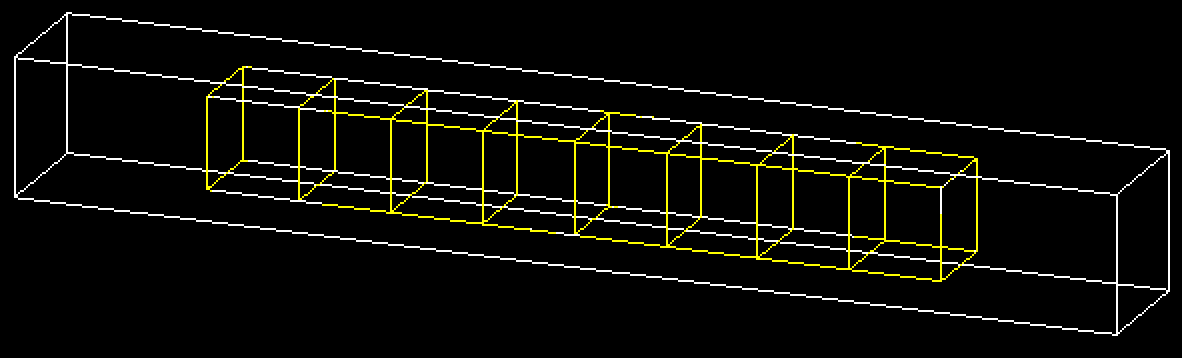
\includegraphics[width=.7\linewidth]{pics/volumes.png}}
\end{frame}

\begin{frame}
  \frametitle{\texttt{PhysicsLists} and \texttt{ActionInitialization/PrimaryGeneratorAction}}
  {\footnotesize
  \begin{itemize}
  \item Physics lists are provided by the Geant4 collaboration.
  \item The collaboration provides descriptions of each physics list which details what kind of physical processes and energy ranges are best for the different lists -- the user then chooses accordingly.
  \item \texttt{G4UserPhysicsList} allows the user to define different particles, processes, and also range cuts of parameters
  \item The user defines the intial state of the system in the \texttt{UserActionInitialization/UserPrimaryGeneratorAction}. What particles should initialize the event, the definition of electric and magnetic fields, etc.
  \item These classes are all derived classes with virtual methods that must be defined by the user for their specific needs!
  \end{itemize}}
\end{frame}

\begin{frame}
  \frametitle{\texttt{RunAction} and \texttt{EventAction}\\(Examples of Optional Classes)}
  \begin{itemize}
  \item A Geant4 run consists of events that all share the same detector, physics, and initial system.
  \item \texttt{RunAction} allows the user to define what occurs at the beginning of a run and at the end of a run using the functions \texttt{RunAction::BeginOfRunAction} and \texttt{RunAction::EndOfRunAction}. The RunAction is made to always call these functions. The user can also create his/her own functions to be called during the run.
  \item \texttt{EventAction} is very similar to RunAction, but of course is initialized $N$ times. 
  \end{itemize}
\end{frame}

\begin{frame}
  \frametitle{Our Modified Example}
  {\footnotesize
  \begin{itemize}
  \item Our simple simulation is based off of \texttt{exampleB4c} from the Geant4 examples.
  \item The example fires a 50 MeV electron into a calorimeter made of a variable number of layers of lead and liquid argon.
  \item B4c yields the total energy deposited and track length in all layers of lead and the total energy deposited in all layers liquid argon combined (no independent layer information). (Using the \texttt{G4Hit} class)
  \item We modified the example in the following way:
    \begin{itemize}
    \item 8 independent ``channels'' (\texttt{G4SensitiveDetectors}) of variable material type (lead, polypropylene, or water) were used in our simple exercise.
    \item Store information on a per layer basis in a \texttt{ROOT} ntuple for each event using a pointer to \texttt{G4RunAction} in \texttt{G4EventAction}.
    \item Particle type and energy modifications. (We used a 2 GeV proton, neutron, muon, and electron)
    \item Two different physics lists were employed. (\texttt{FTFP\_BERT}, \texttt{QGSP\_BERT}).
    \item All 24 scenarios were run with 10,000 events each.
    \end{itemize}
  \end{itemize}}
\end{frame}

\begin{frame}
  \frametitle{Our Modified Example cont'd}
  {\footnotesize
  \begin{itemize}
    \item Distributions of E\textsubscript{deposited} and average track length per layer were created from each layers sensitive detector readout.
    \item Both physics lists produced identical results for the energies, materials, and particles considered. Therefore, we'll discuss 12 systems in the simple analysis of the upcoming slides.
    \item The following plots were all created from simulations using the \texttt{FTFP\_BERT} physics list.
  \end{itemize}}
\end{frame}

% electron
\begin{frame}
  \frametitle{Electron Interactions}
  \begin{picture}(320,250)(-160,-125)
  \put(-160, 60){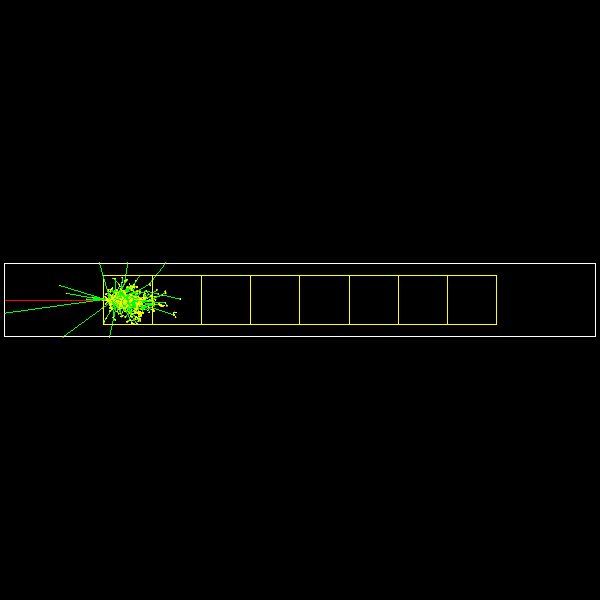
\includegraphics[width=.48\textwidth, trim = 0mm 75mm 0mm 75mm, clip]{../report/pics/e-Pb.png}}
  \put(-160, -60){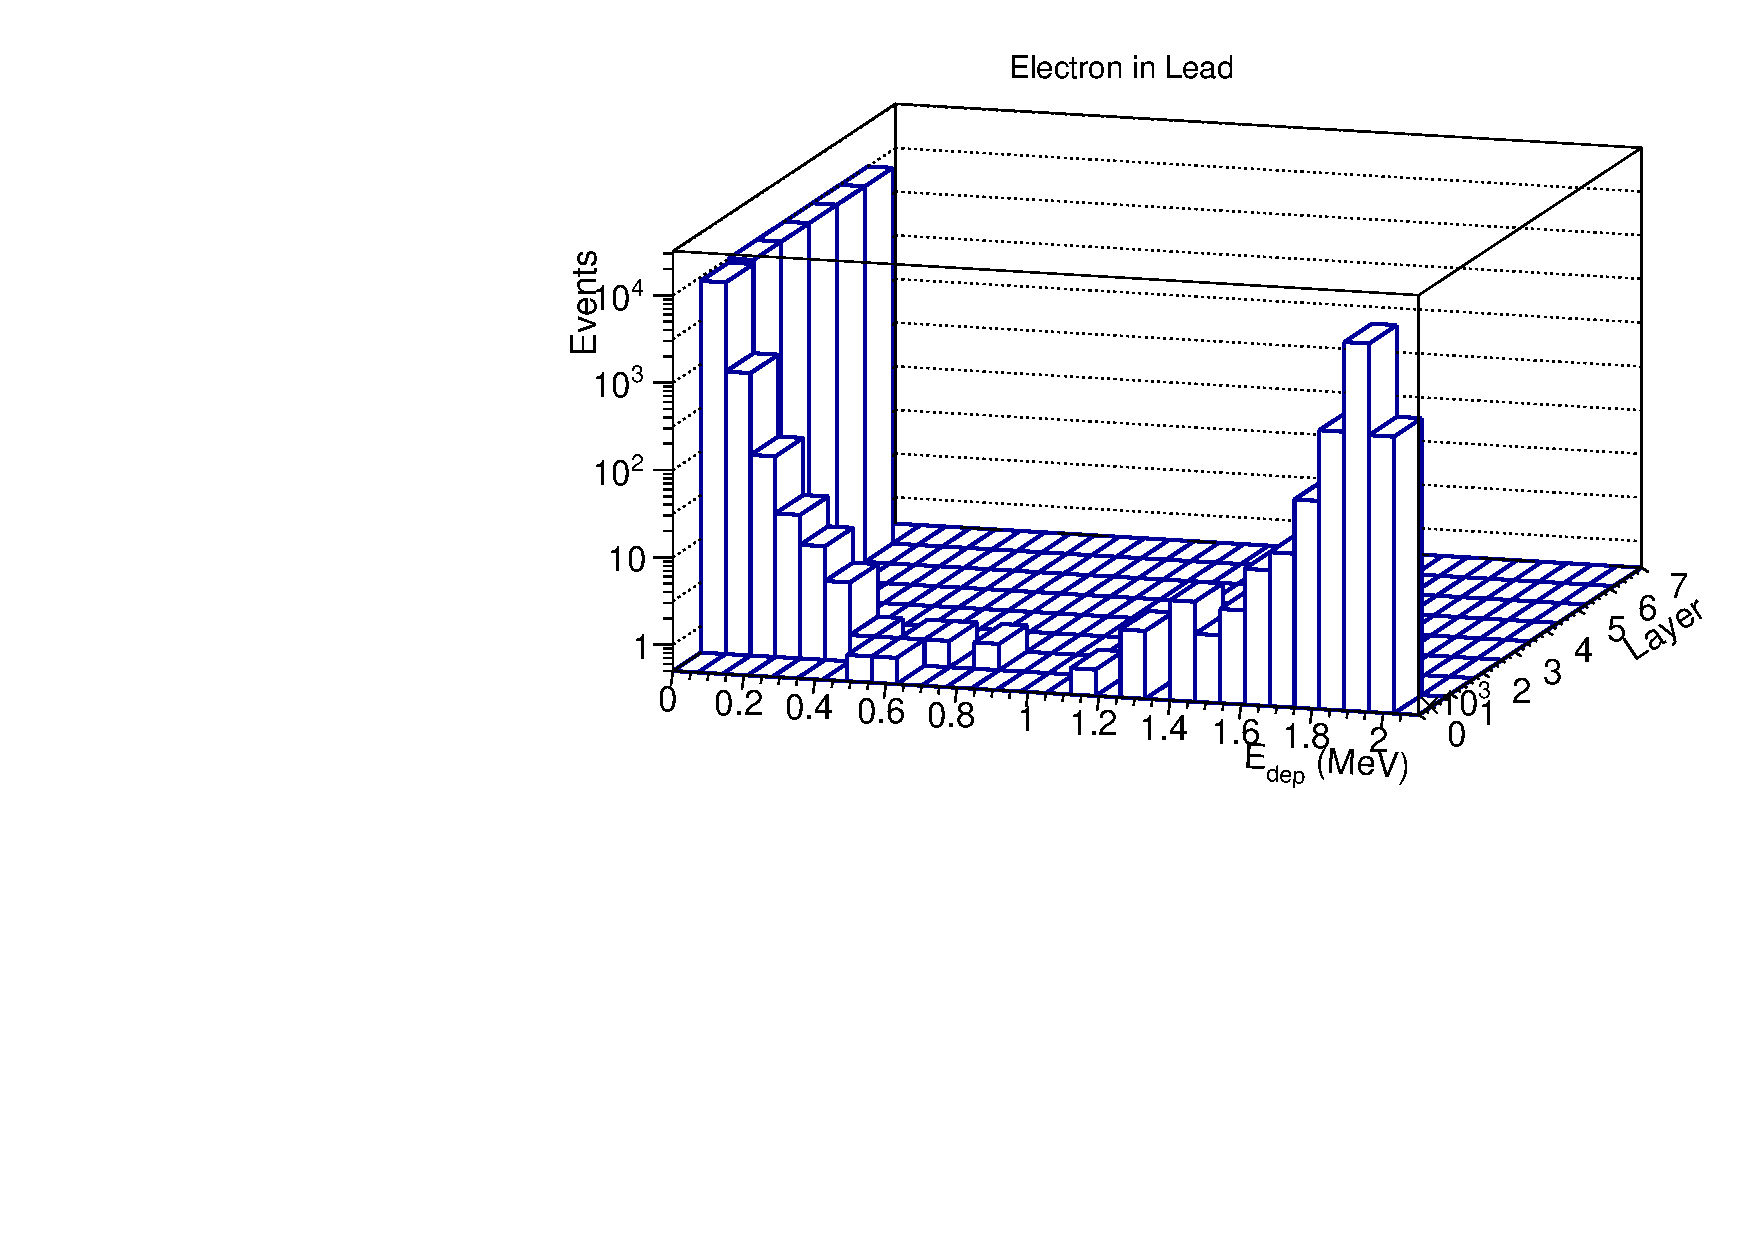
\includegraphics[width=.48\textwidth]{../report/plots/electron_pb_edep.pdf}}
  \put(18.5, 60){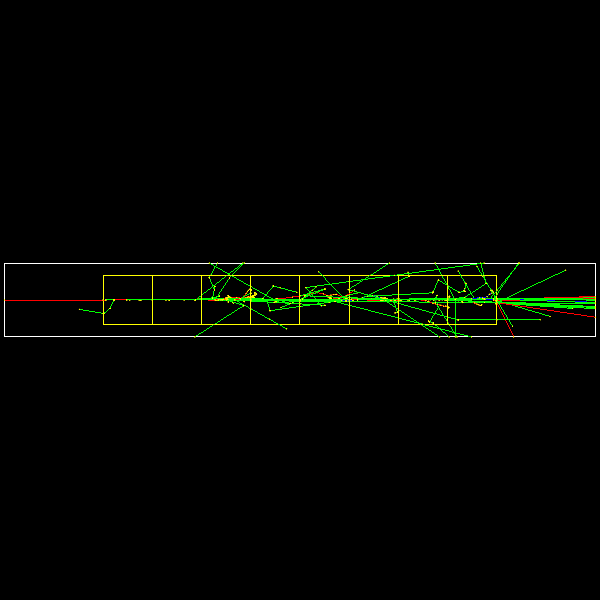
\includegraphics[width=.48\textwidth, trim = 0mm 75mm 0mm 75mm, clip]{../report/pics/e-PP.png}}
  \put(18.5, -60){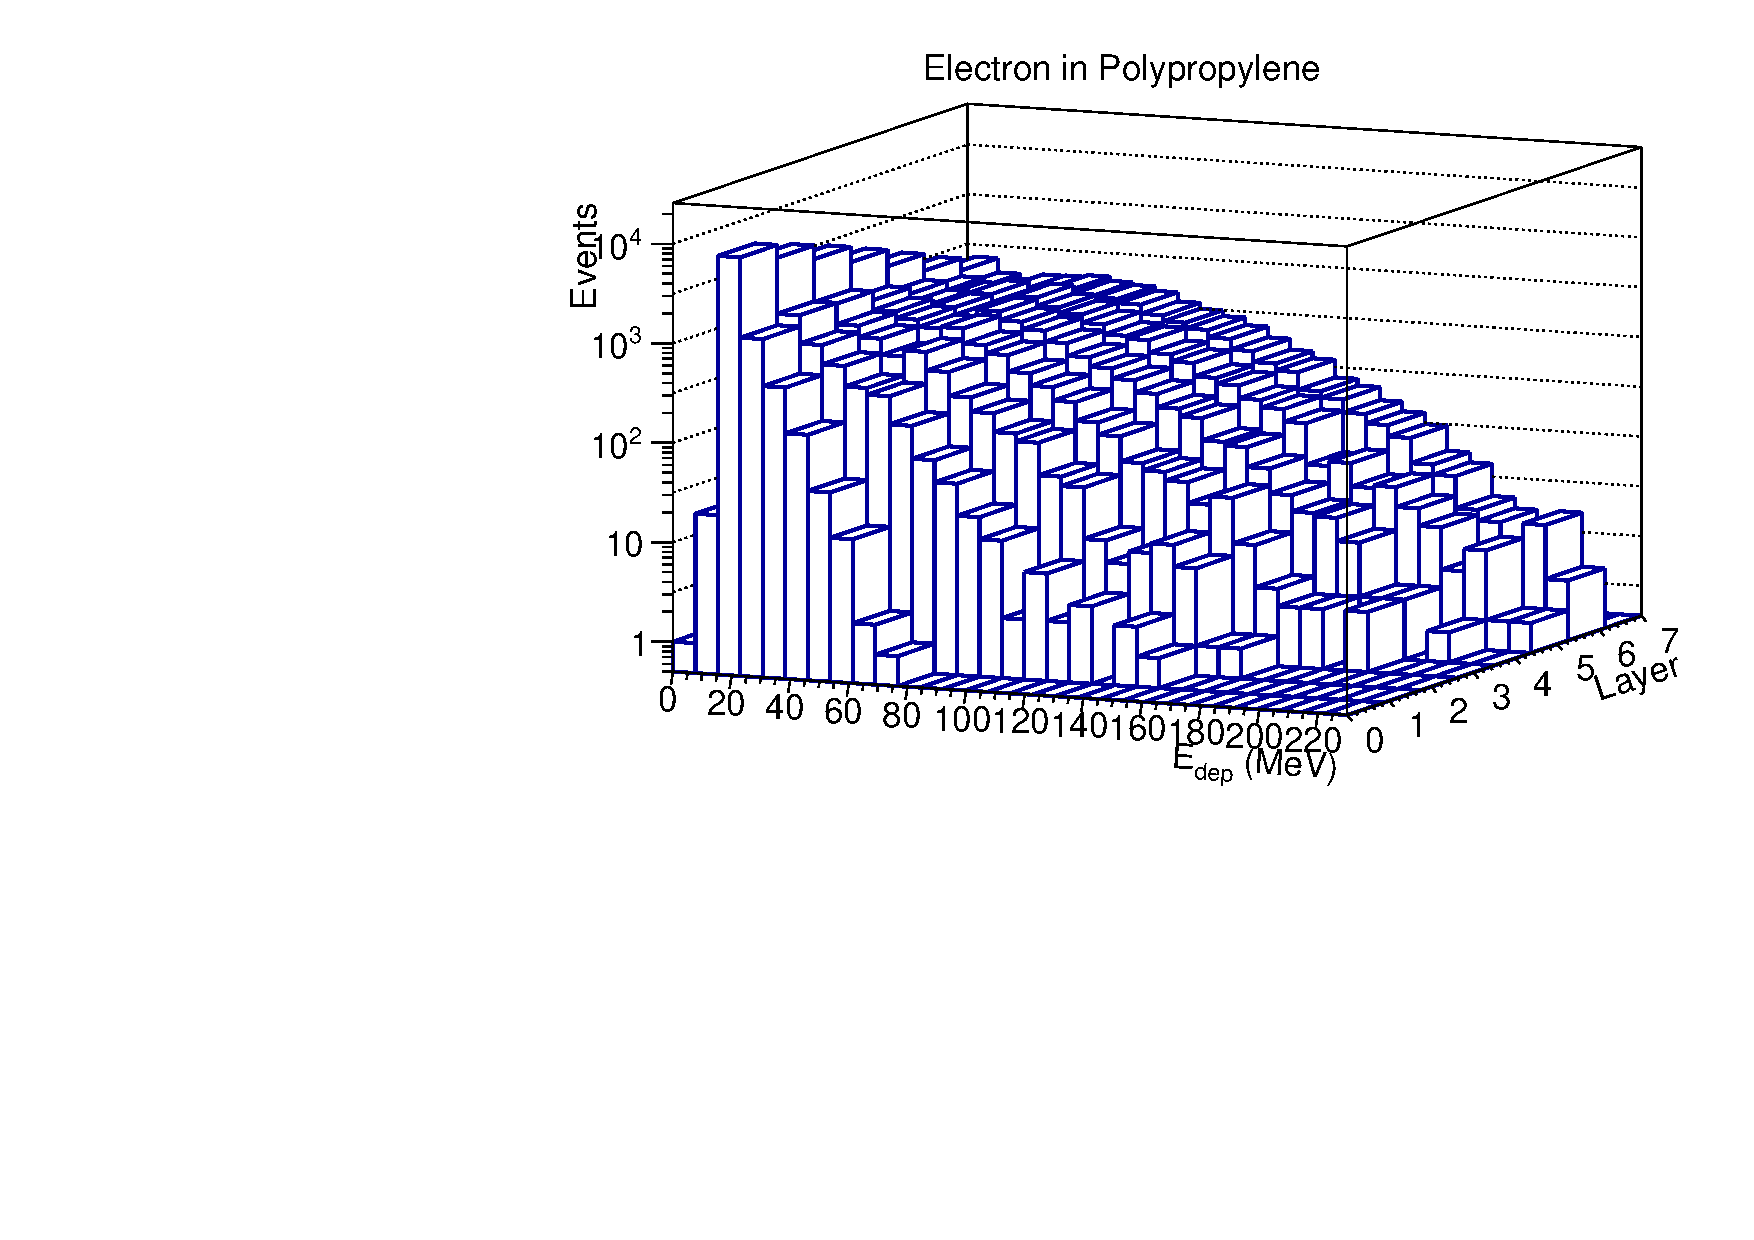
\includegraphics[width=.48\textwidth]{../report/plots/electron_pp_edep.pdf}}
  \end{picture}
\end{frame}

\begin{frame}
  \frametitle{Electron Interactions cont'd}
  \begin{picture}(320,250)(-160,-125)
  \put(-160, 60){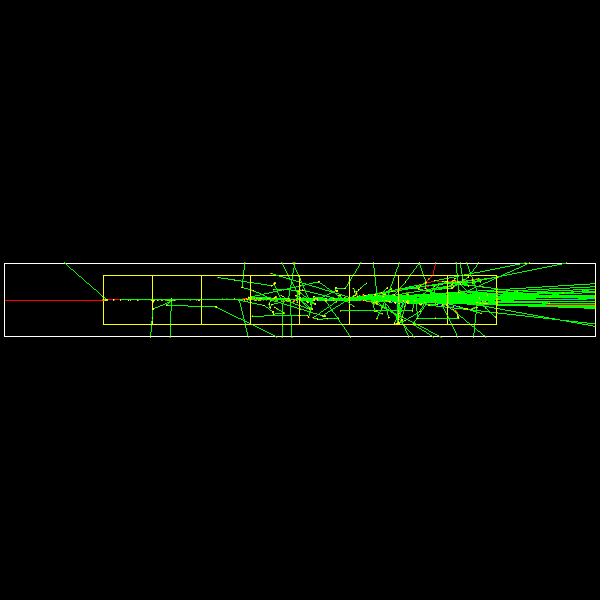
\includegraphics[width=.48\textwidth, trim = 0mm 75mm 0mm 75mm, clip]{../report/pics/e-H2O.png}}
  \put(-160, -60){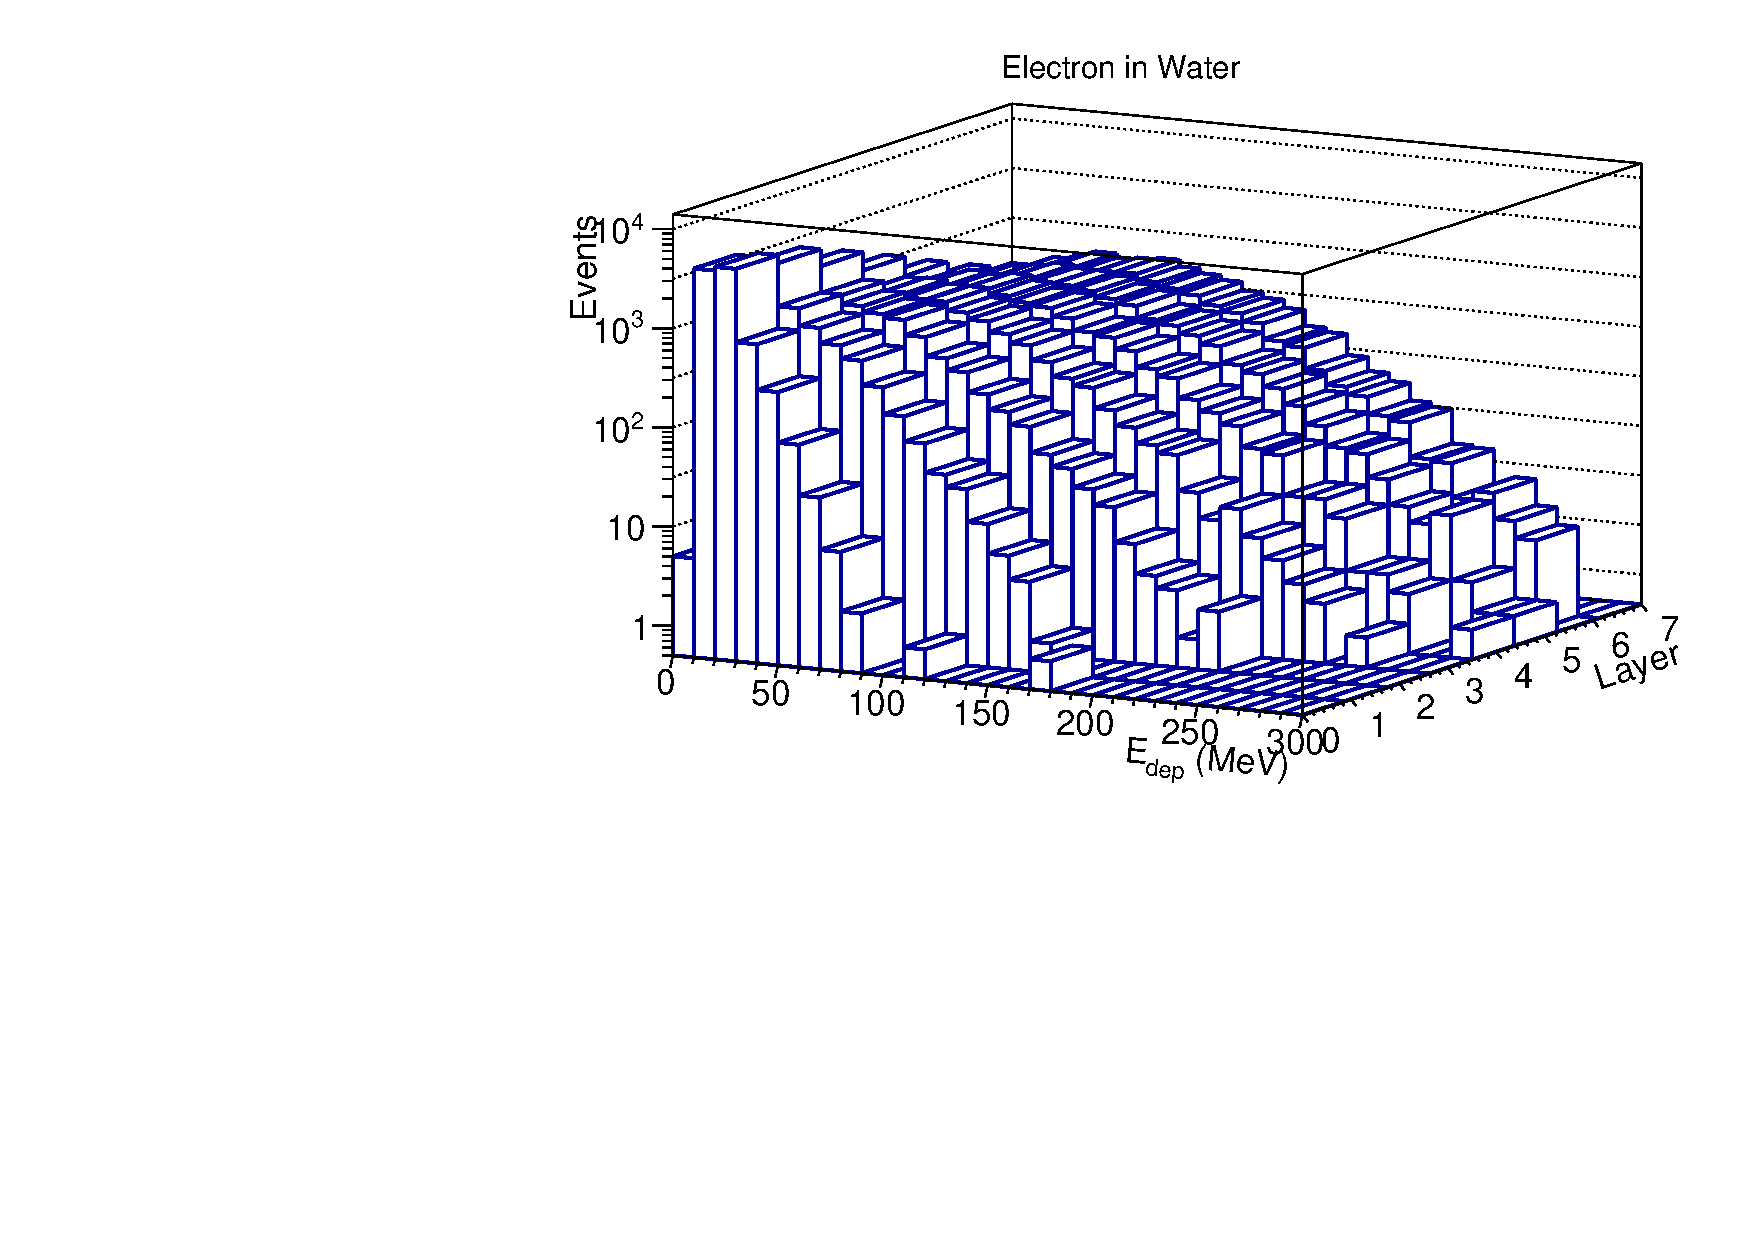
\includegraphics[width=.48\textwidth]{../report/plots/electron_h2o_edep.pdf}}
  \put(18.5, -30){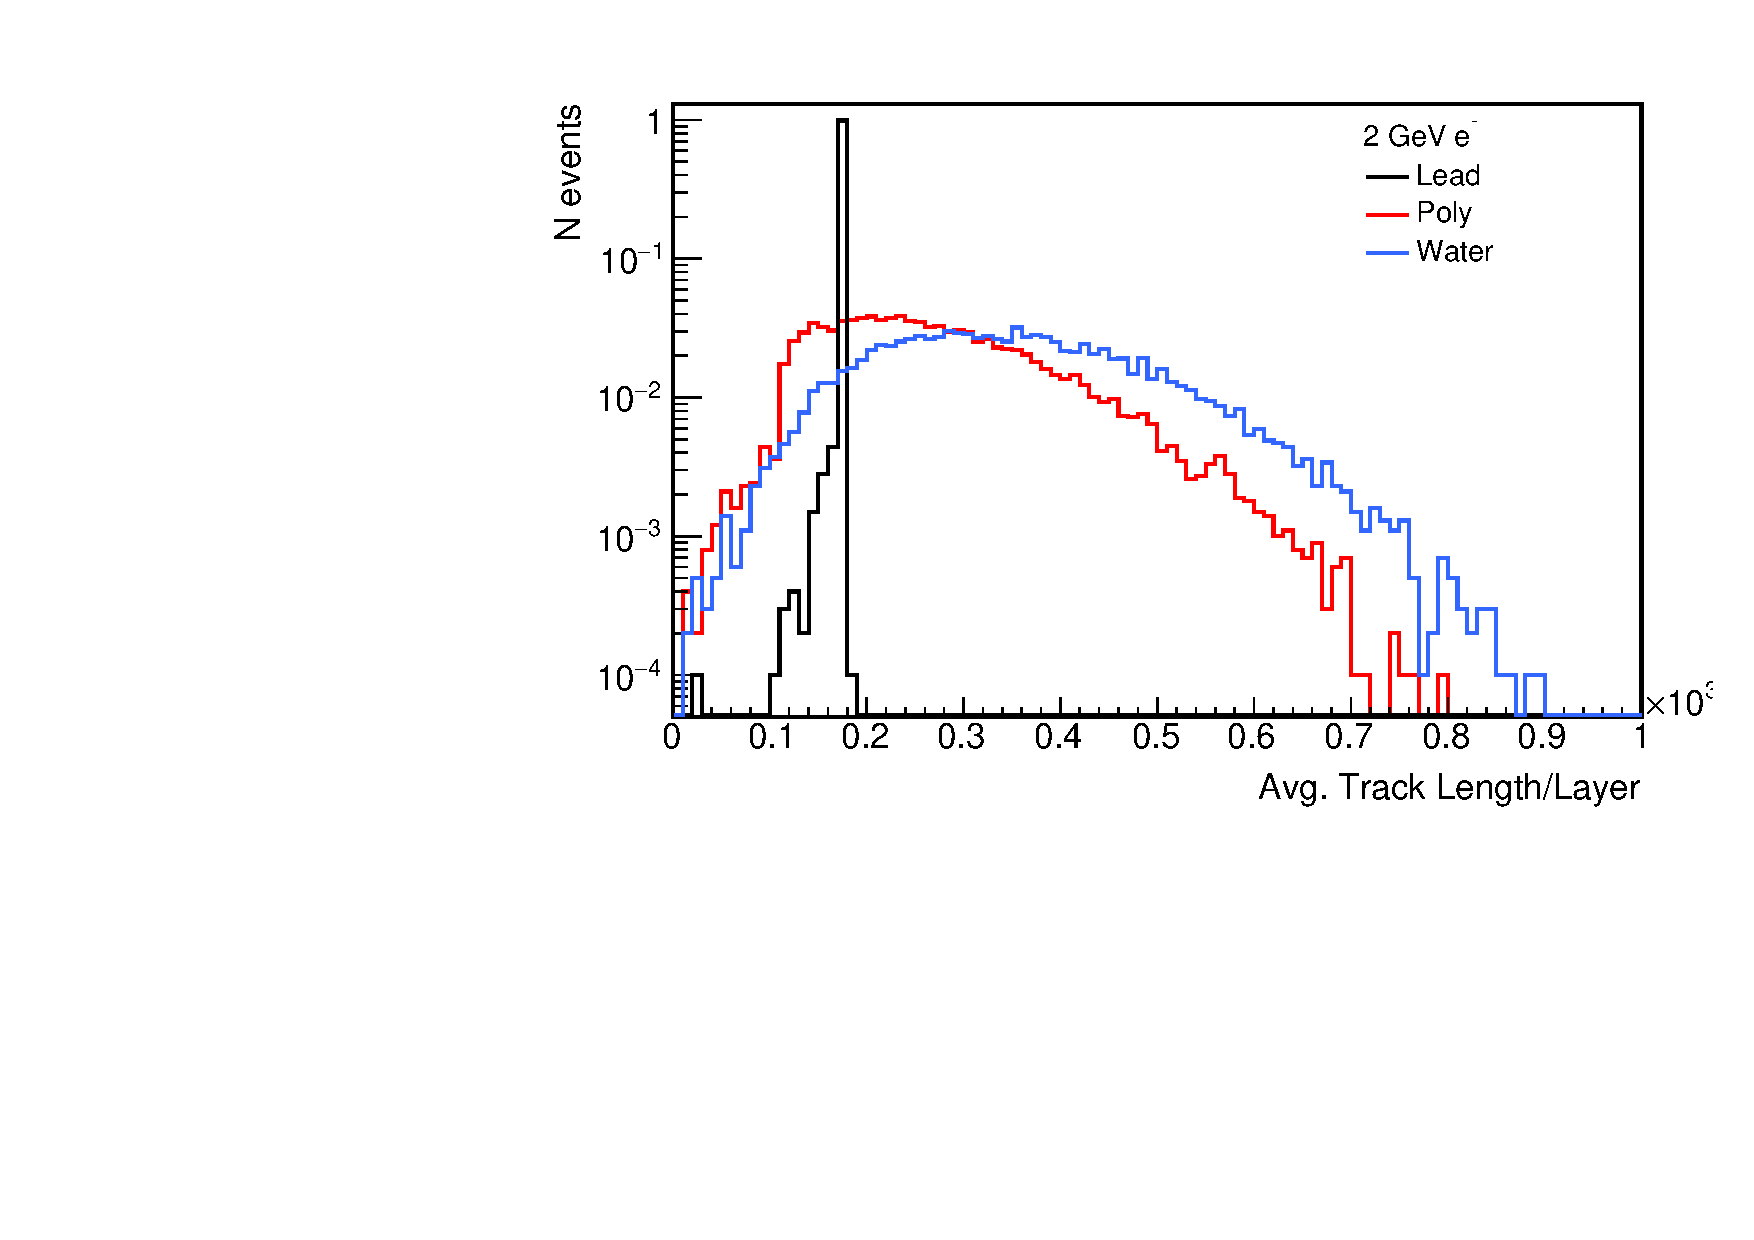
\includegraphics[width=.48\textwidth]{../report/plots/TL_electron.pdf}}
  \end{picture}
\end{frame}

% muon
\begin{frame}
  \frametitle{Muon Interactions}
  \begin{picture}(320,250)(-160,-125)
  \put(-160, 60){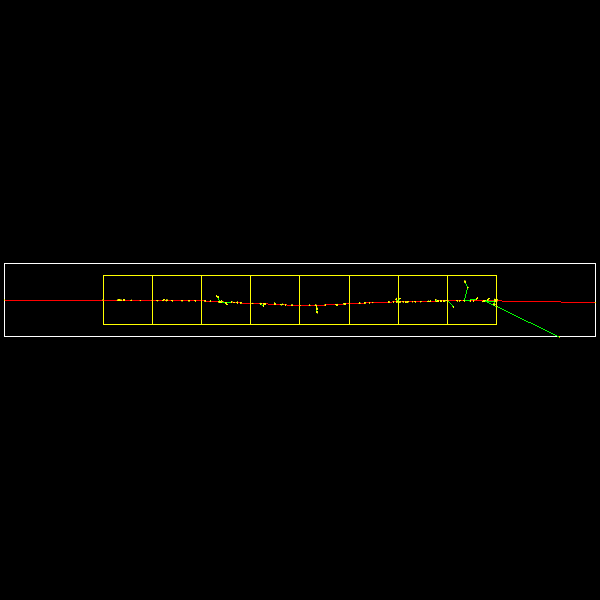
\includegraphics[width=.48\textwidth, trim = 0mm 75mm 0mm 75mm, clip]{../report/pics/mu-Pb.png}}
  \put(-160, -60){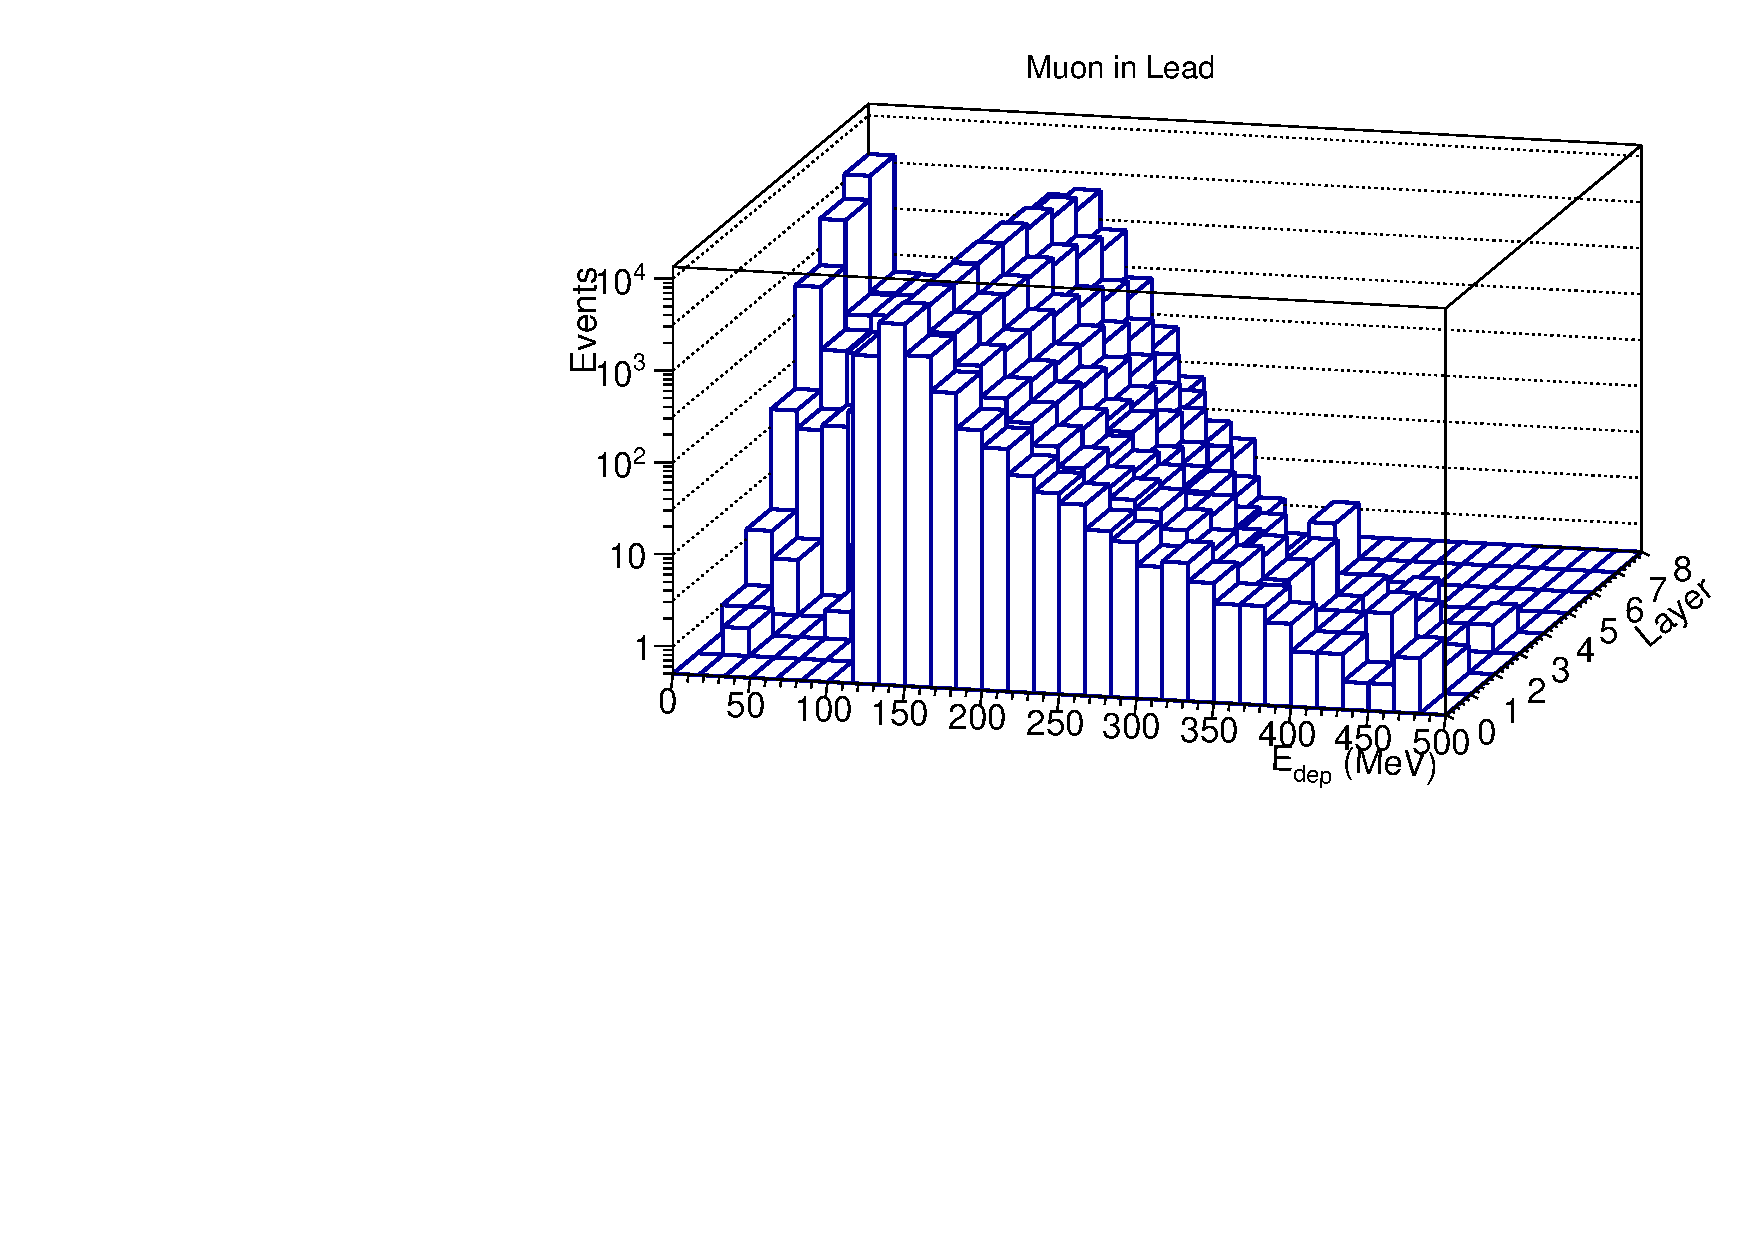
\includegraphics[width=.48\textwidth]{../report/plots/muon_pb_edep.pdf}}
  \put(18.5, 60){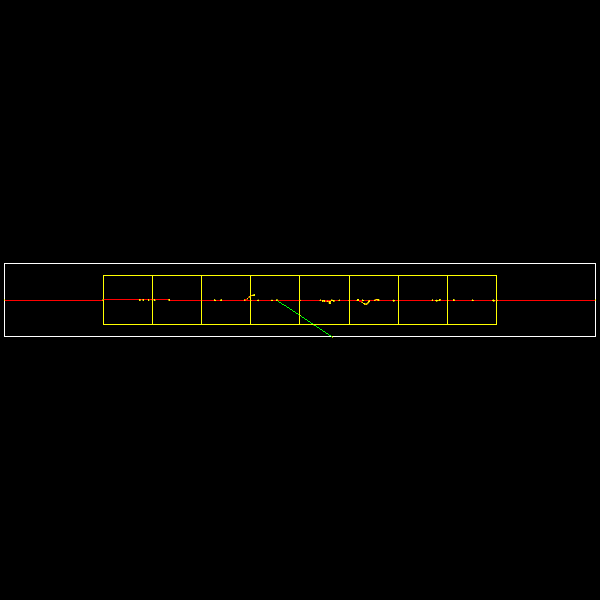
\includegraphics[width=.48\textwidth, trim = 0mm 75mm 0mm 75mm, clip]{../report/pics/mu-PP.png}}
  \put(18.5, -60){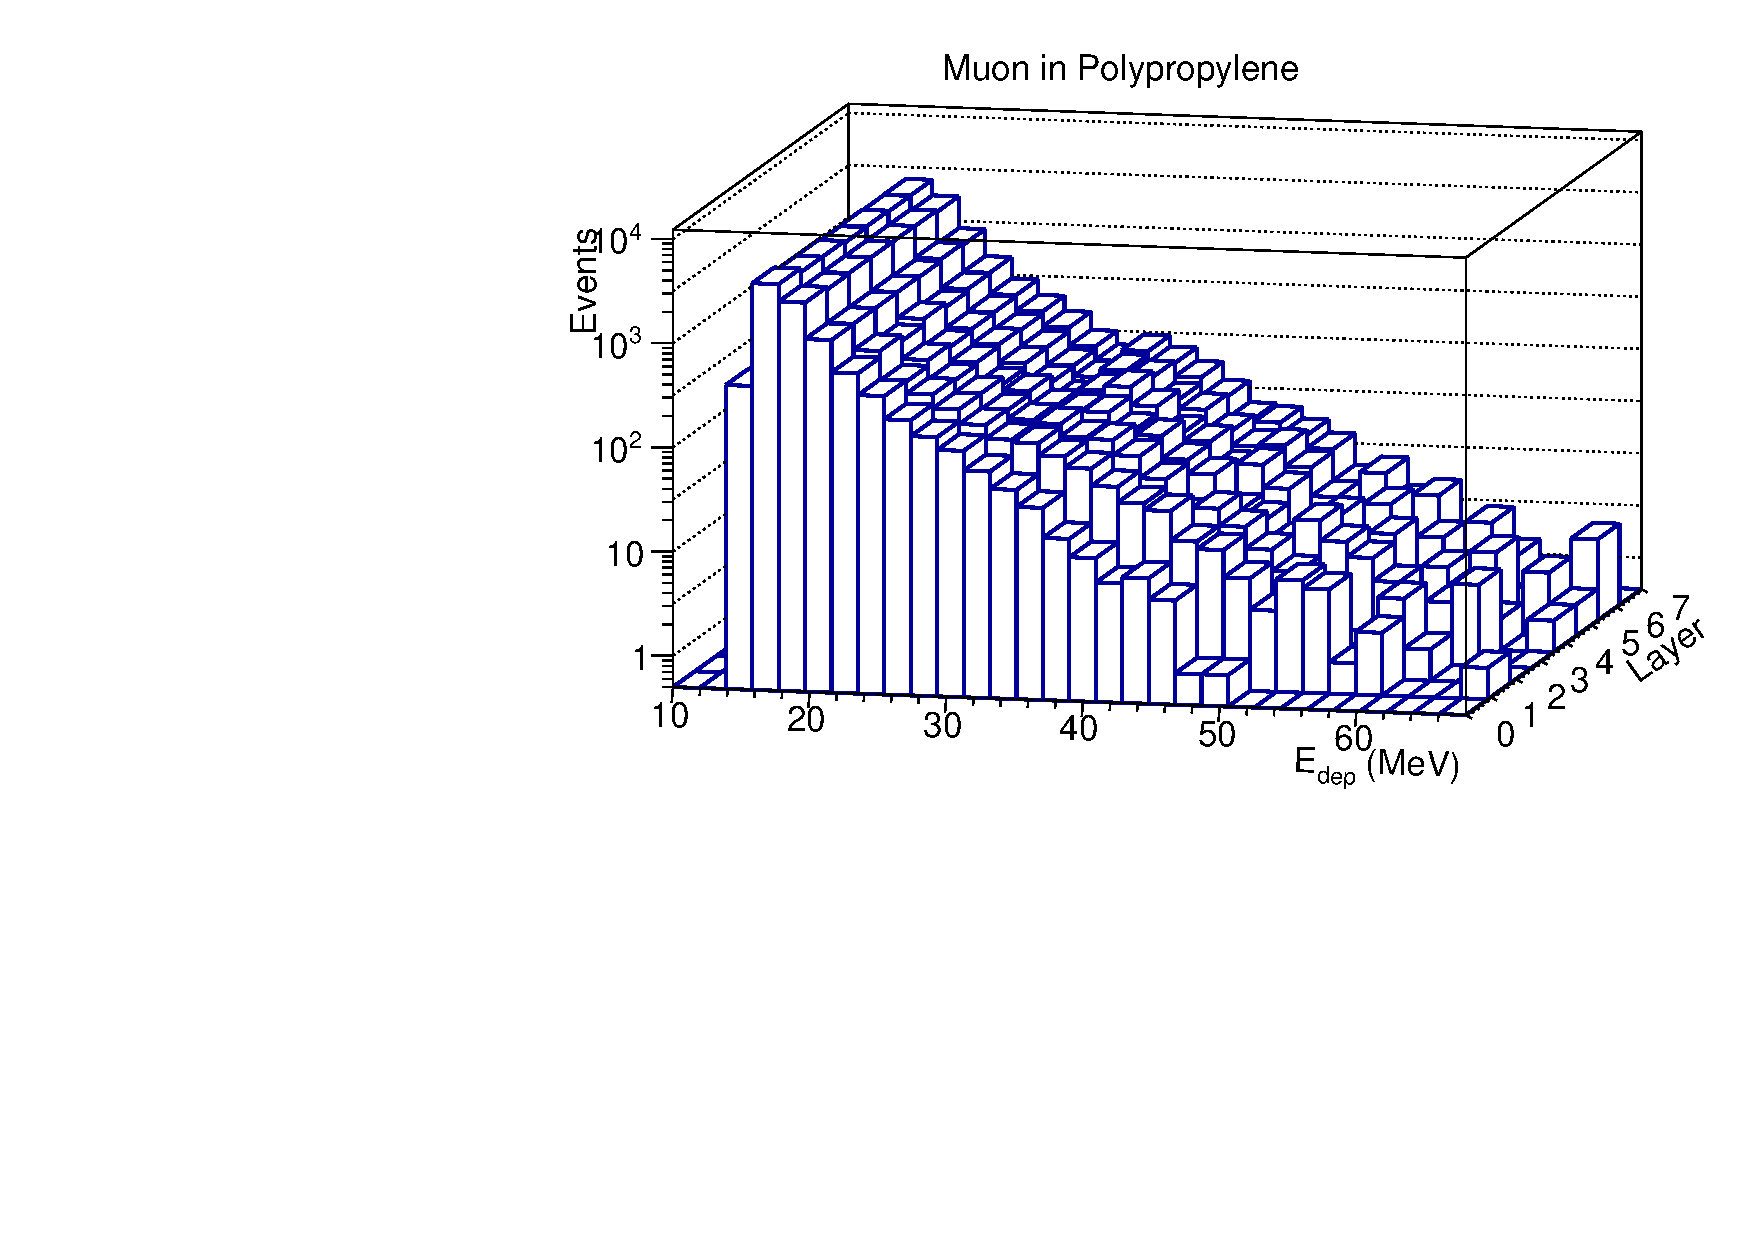
\includegraphics[width=.48\textwidth]{../report/plots/muon_pp_edep.pdf}}
  \end{picture}
\end{frame}

\begin{frame}
  \frametitle{Muon Interactions cont'd}
  \begin{picture}(320,250)(-160,-125)
  \put(-160, 60){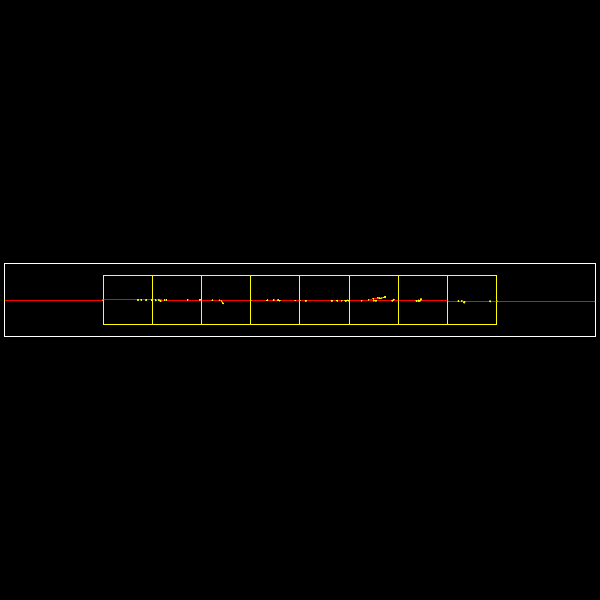
\includegraphics[width=.48\textwidth, trim = 0mm 75mm 0mm 75mm, clip]{../report/pics/mu-H2O.png}}
  \put(-160, -60){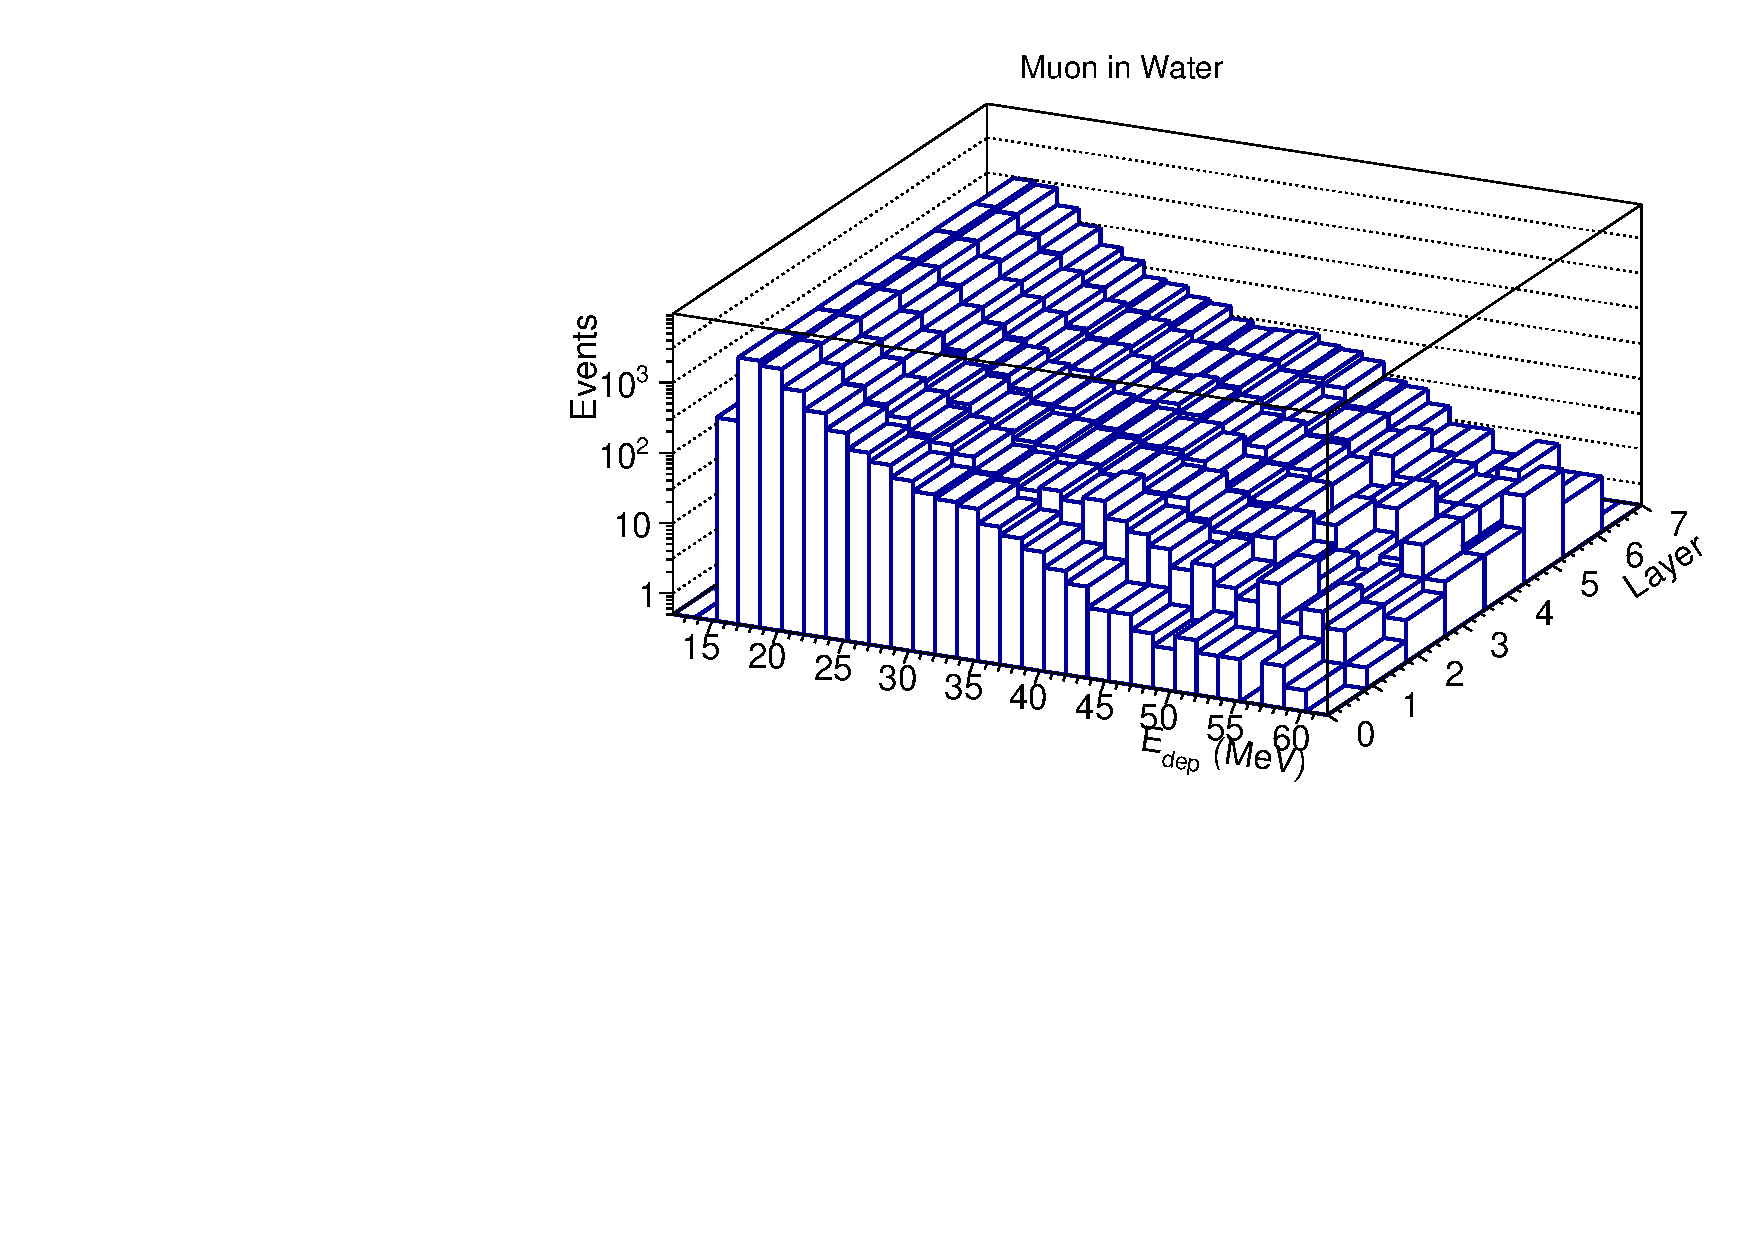
\includegraphics[width=.48\textwidth]{../report/plots/muon_h2o_edep.pdf}}
  \put(18.5, -30){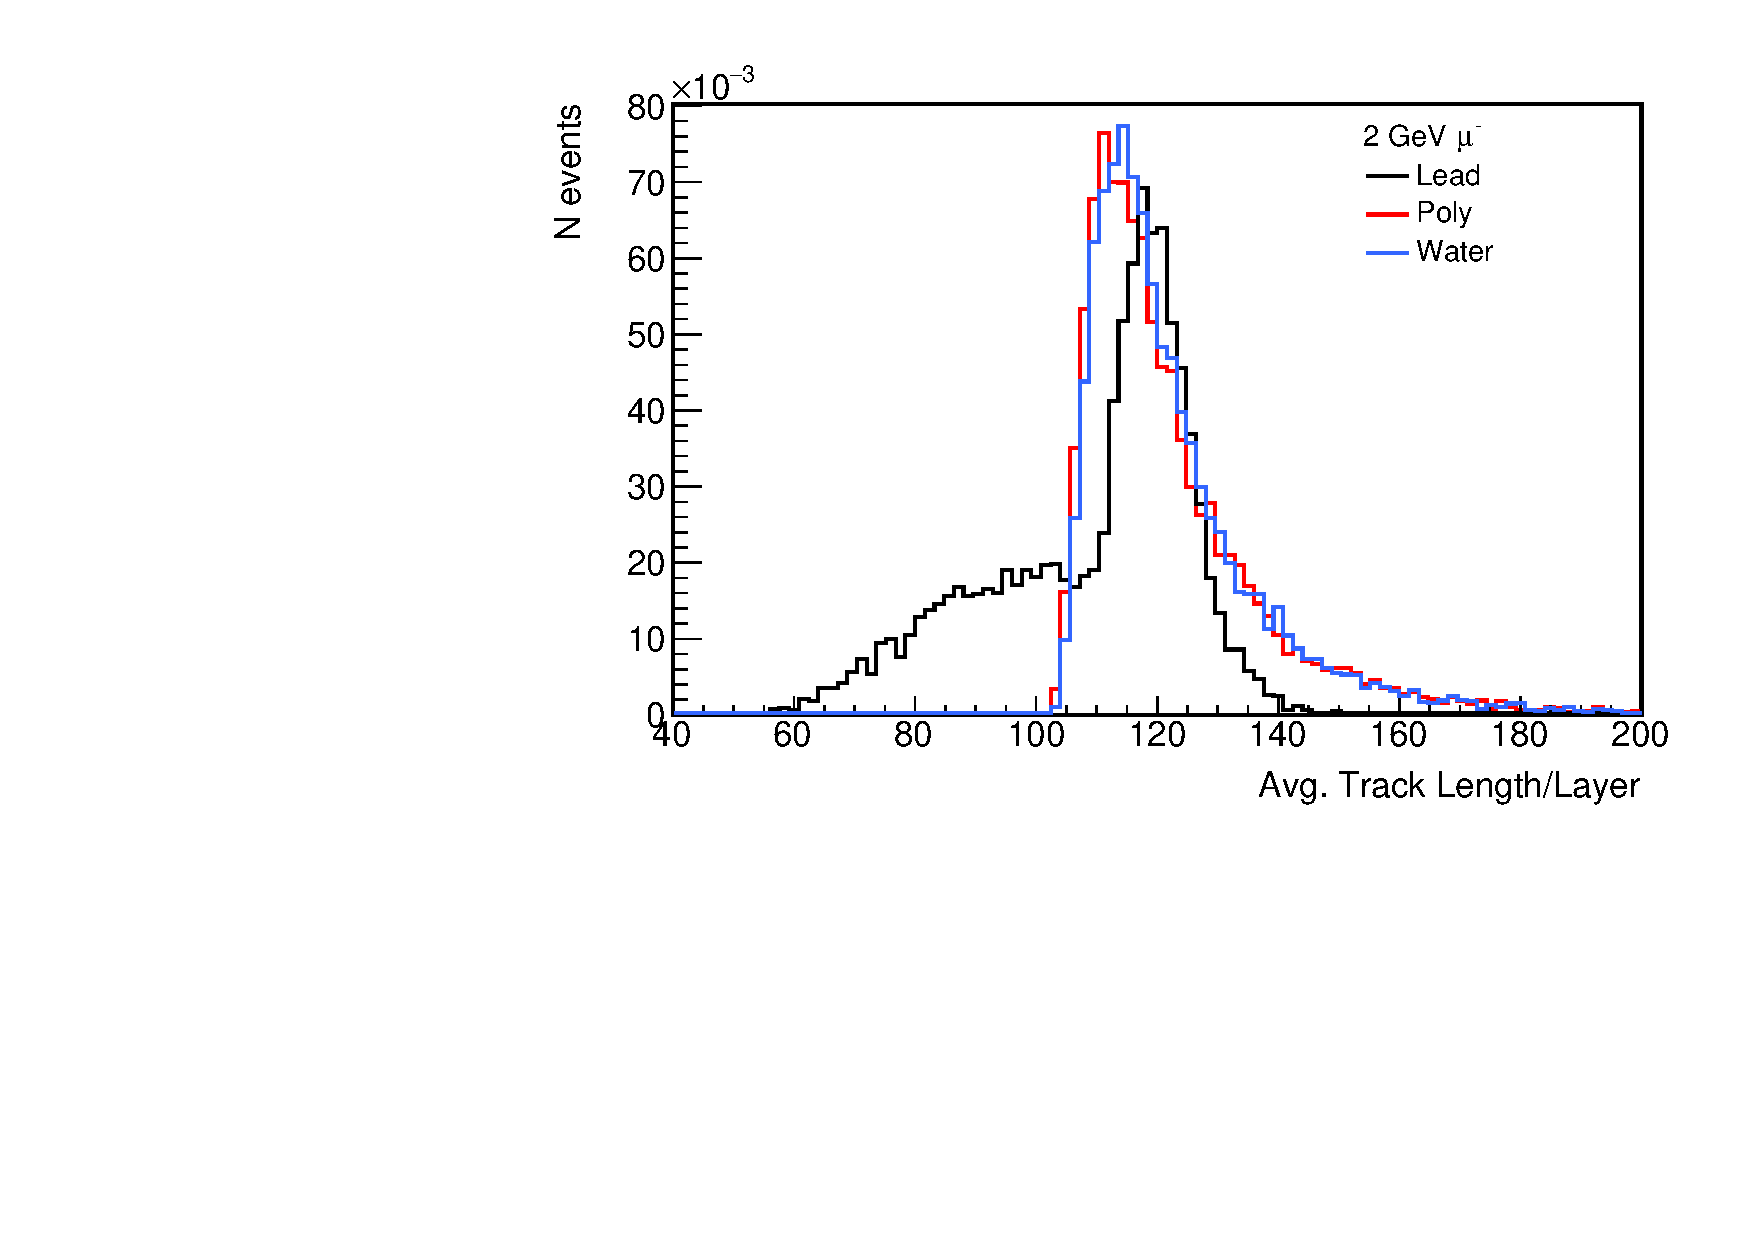
\includegraphics[width=.48\textwidth]{../report/plots/TL_muon.pdf}}
  \end{picture}
\end{frame}

% proton
\begin{frame}
  \frametitle{Proton Interactions}
  \begin{picture}(320,250)(-160,-125)
  \put(-160, 60){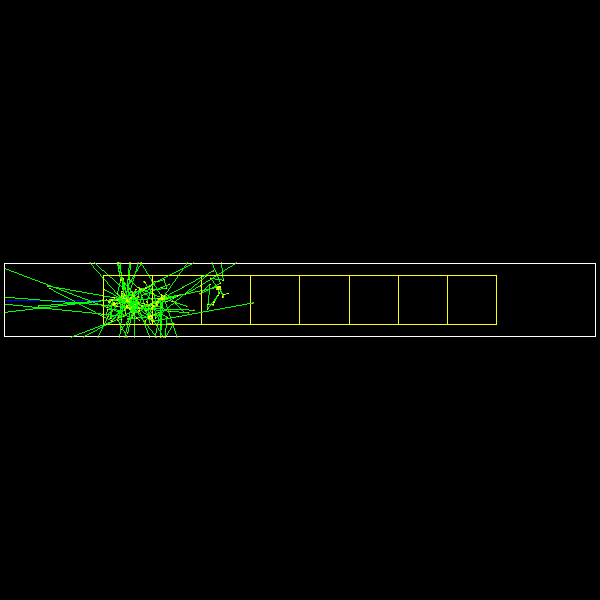
\includegraphics[width=.48\textwidth, trim = 0mm 75mm 0mm 75mm, clip]{../report/pics/P-Pb.png}}
  \put(-160, -60){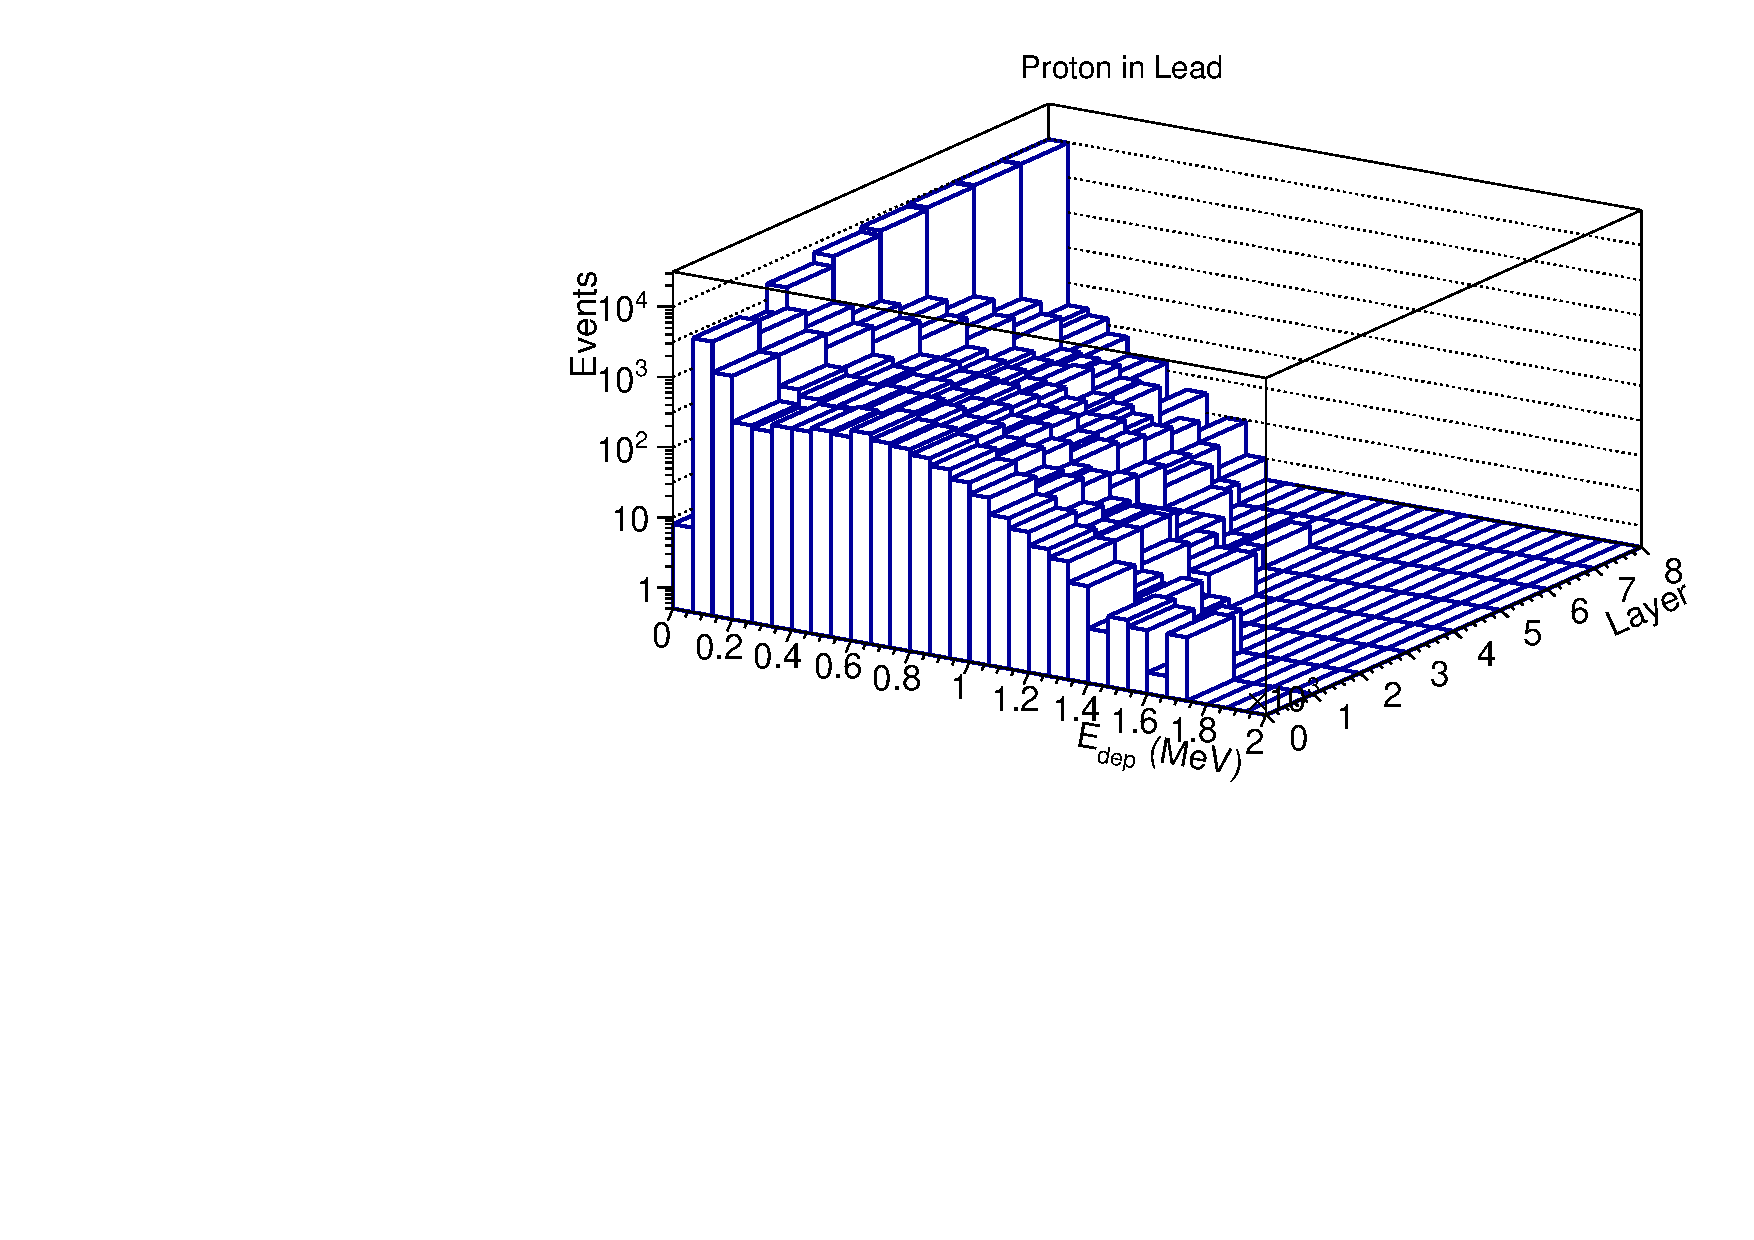
\includegraphics[width=.48\textwidth]{../report/plots/P_pb_edep.pdf}}
  \put(18.5, 60){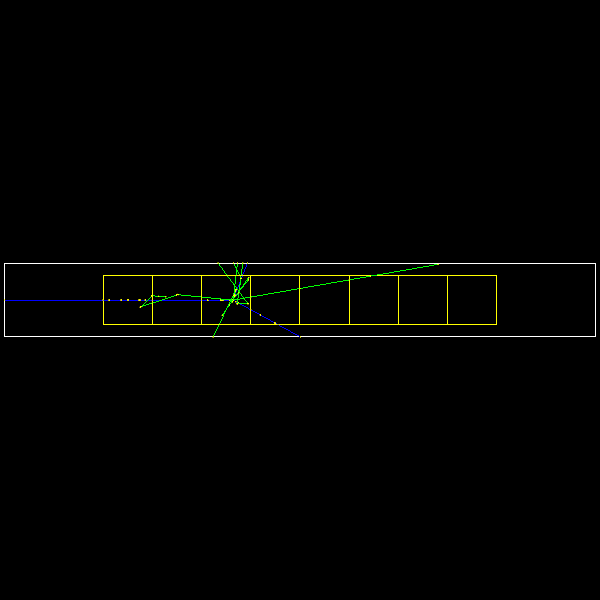
\includegraphics[width=.48\textwidth, trim = 0mm 75mm 0mm 75mm, clip]{../report/pics/P-PP.png}}
  \put(18.5, -60){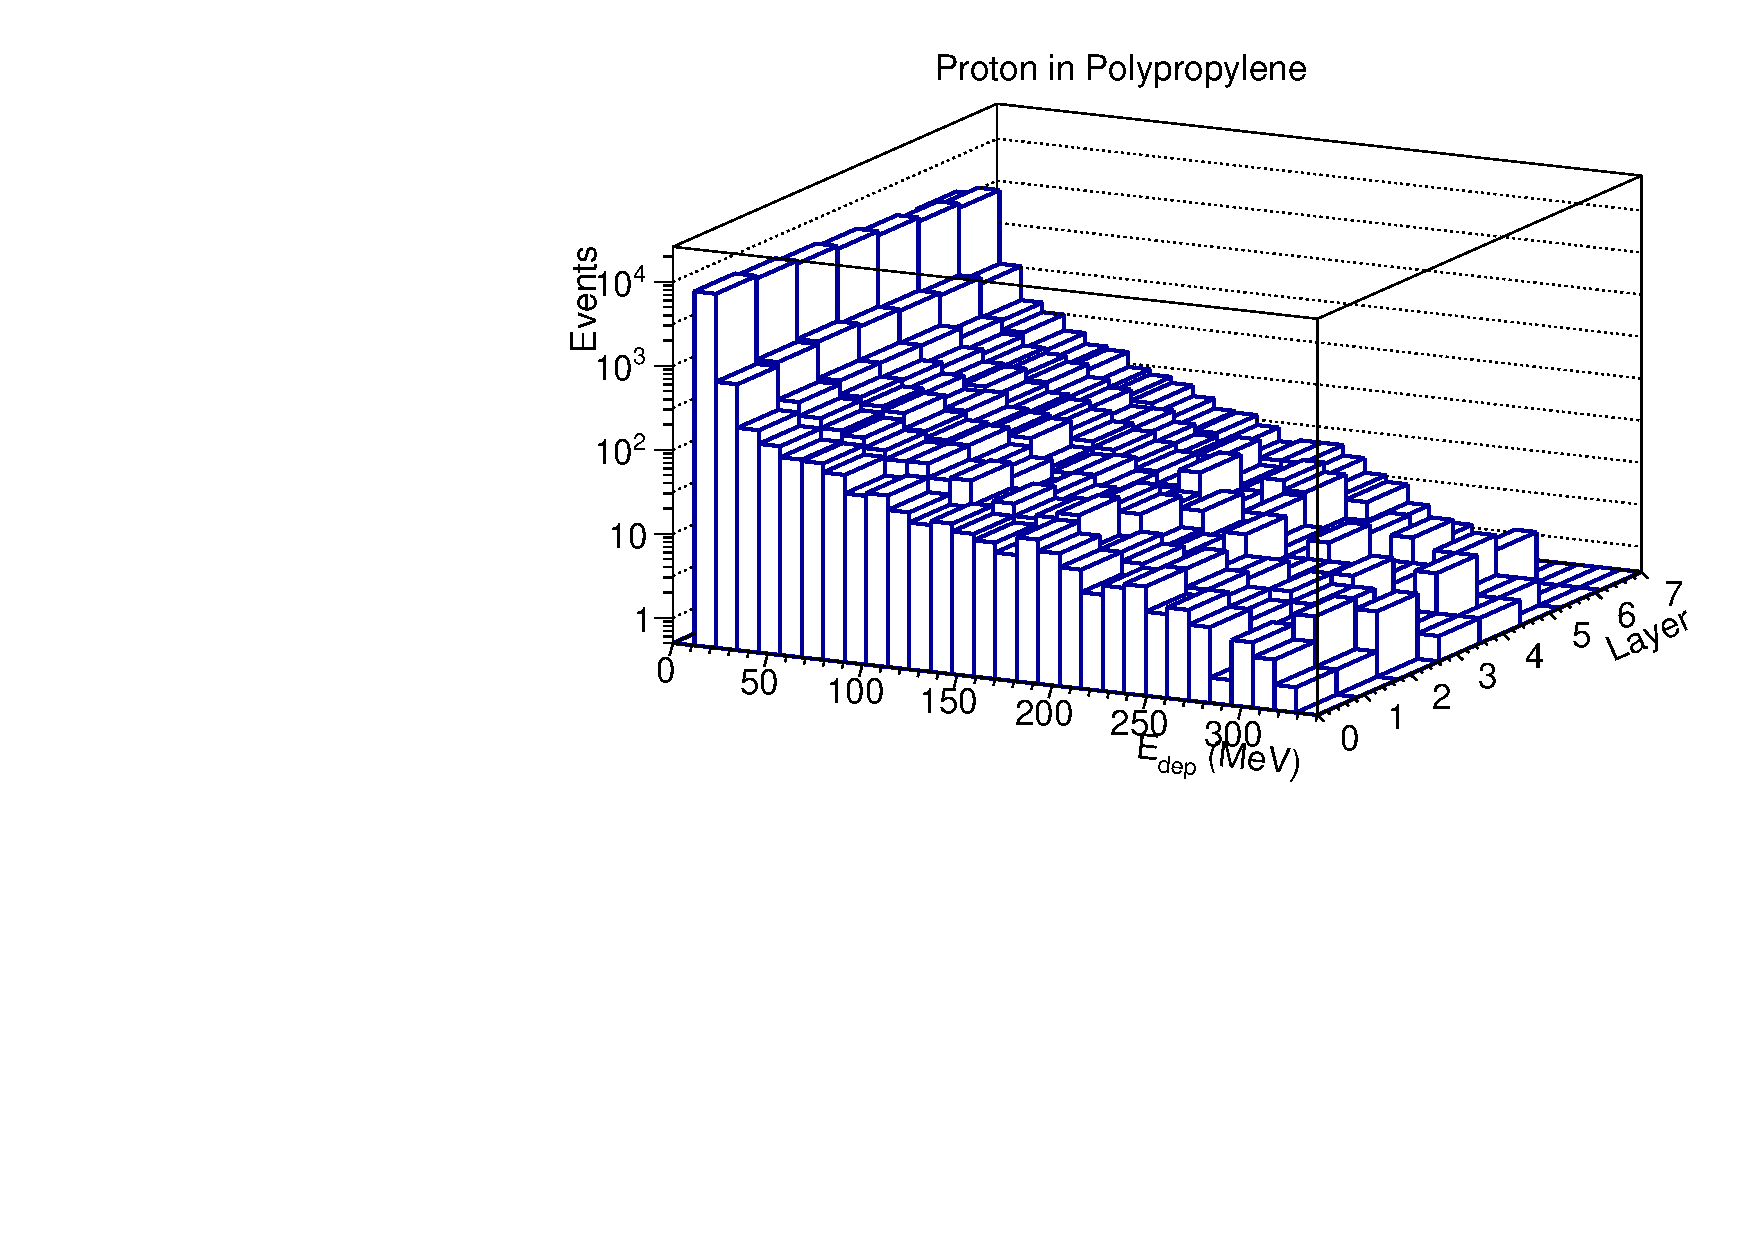
\includegraphics[width=.48\textwidth]{../report/plots/P_pp_edep.pdf}}
  \end{picture}
\end{frame}

\begin{frame}
  \frametitle{Proton Interactions cont'd}
  \begin{picture}(320,250)(-160,-125)
  \put(-160, 60){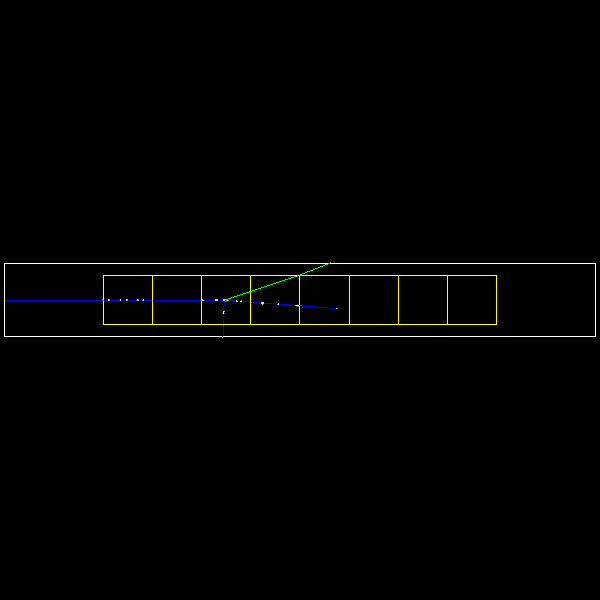
\includegraphics[width=.48\textwidth, trim = 0mm 75mm 0mm 75mm, clip]{../report/pics/P-H2O.png}}
  \put(-160, -60){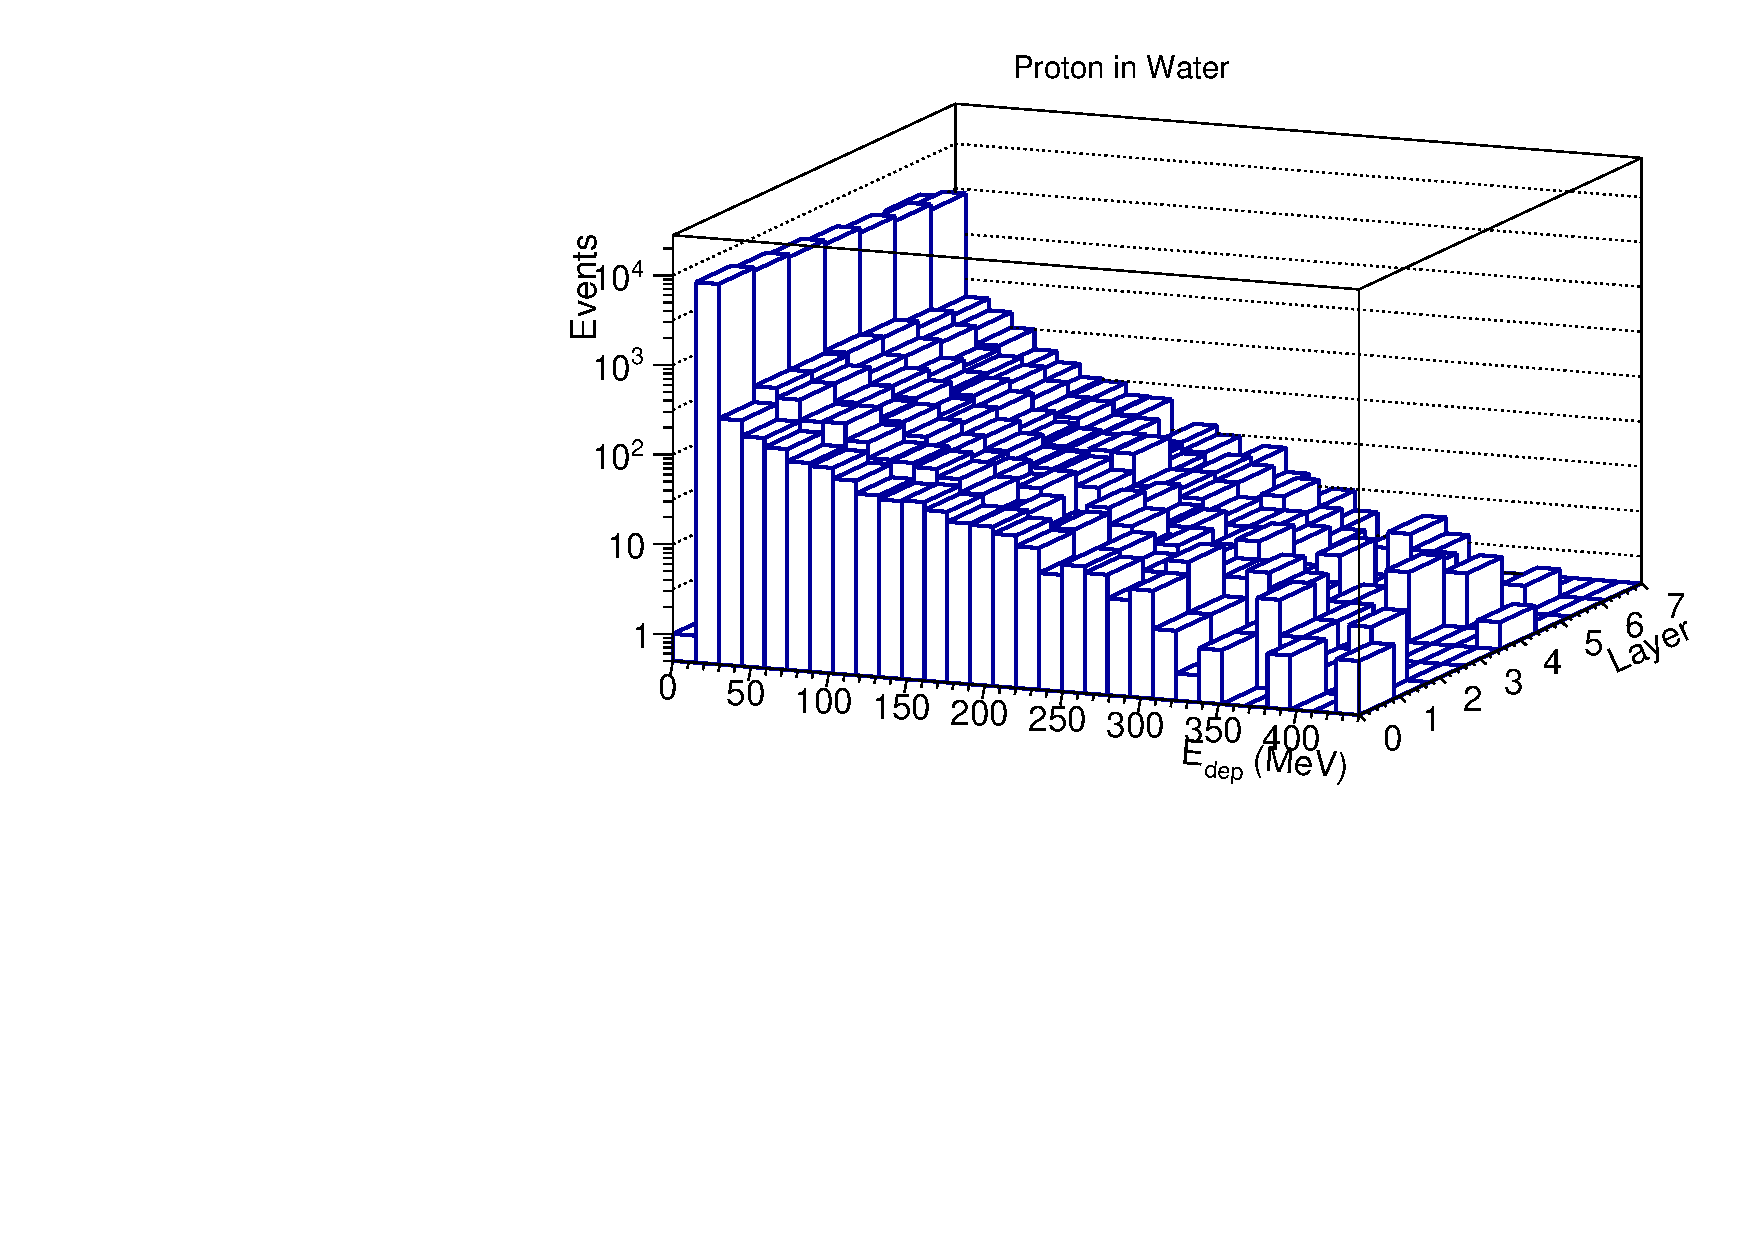
\includegraphics[width=.48\textwidth]{../report/plots/P_h2o_edep.pdf}}
  \put(18.5, -30){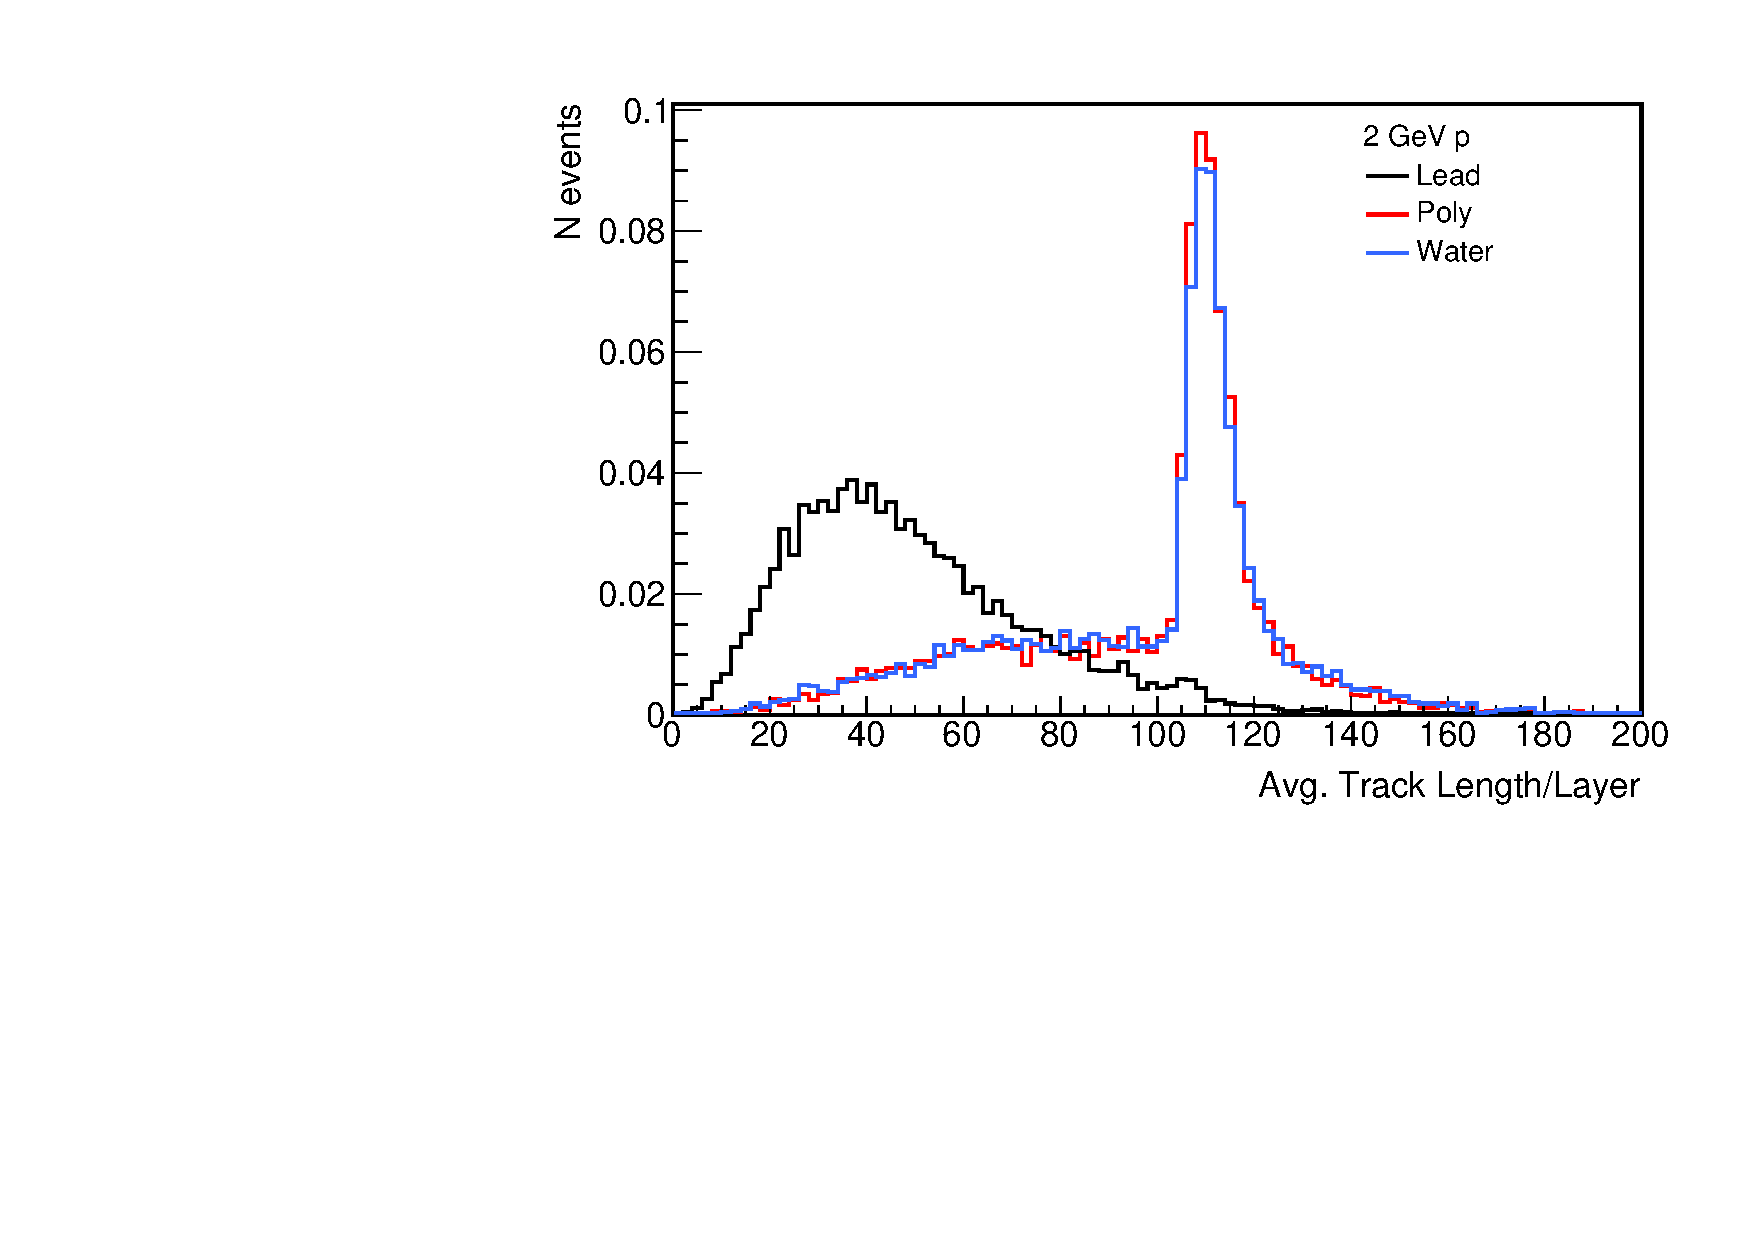
\includegraphics[width=.48\textwidth]{../report/plots/TL_proton.pdf}}
  \end{picture}
\end{frame}

% neutron
\begin{frame}
  \frametitle{Neutron Interactions}
  \begin{picture}(320,250)(-160,-125)
  \put(-160, 60){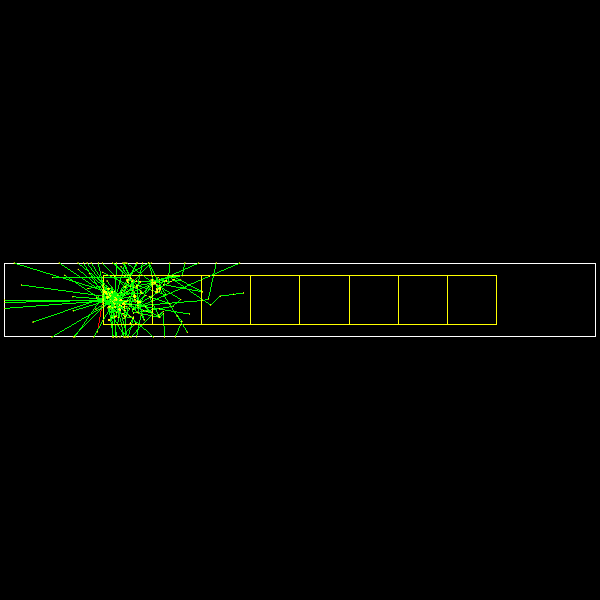
\includegraphics[width=.48\textwidth, trim = 0mm 75mm 0mm 75mm, clip]{../report/pics/N-Pb.png}}
  \put(-160, -60){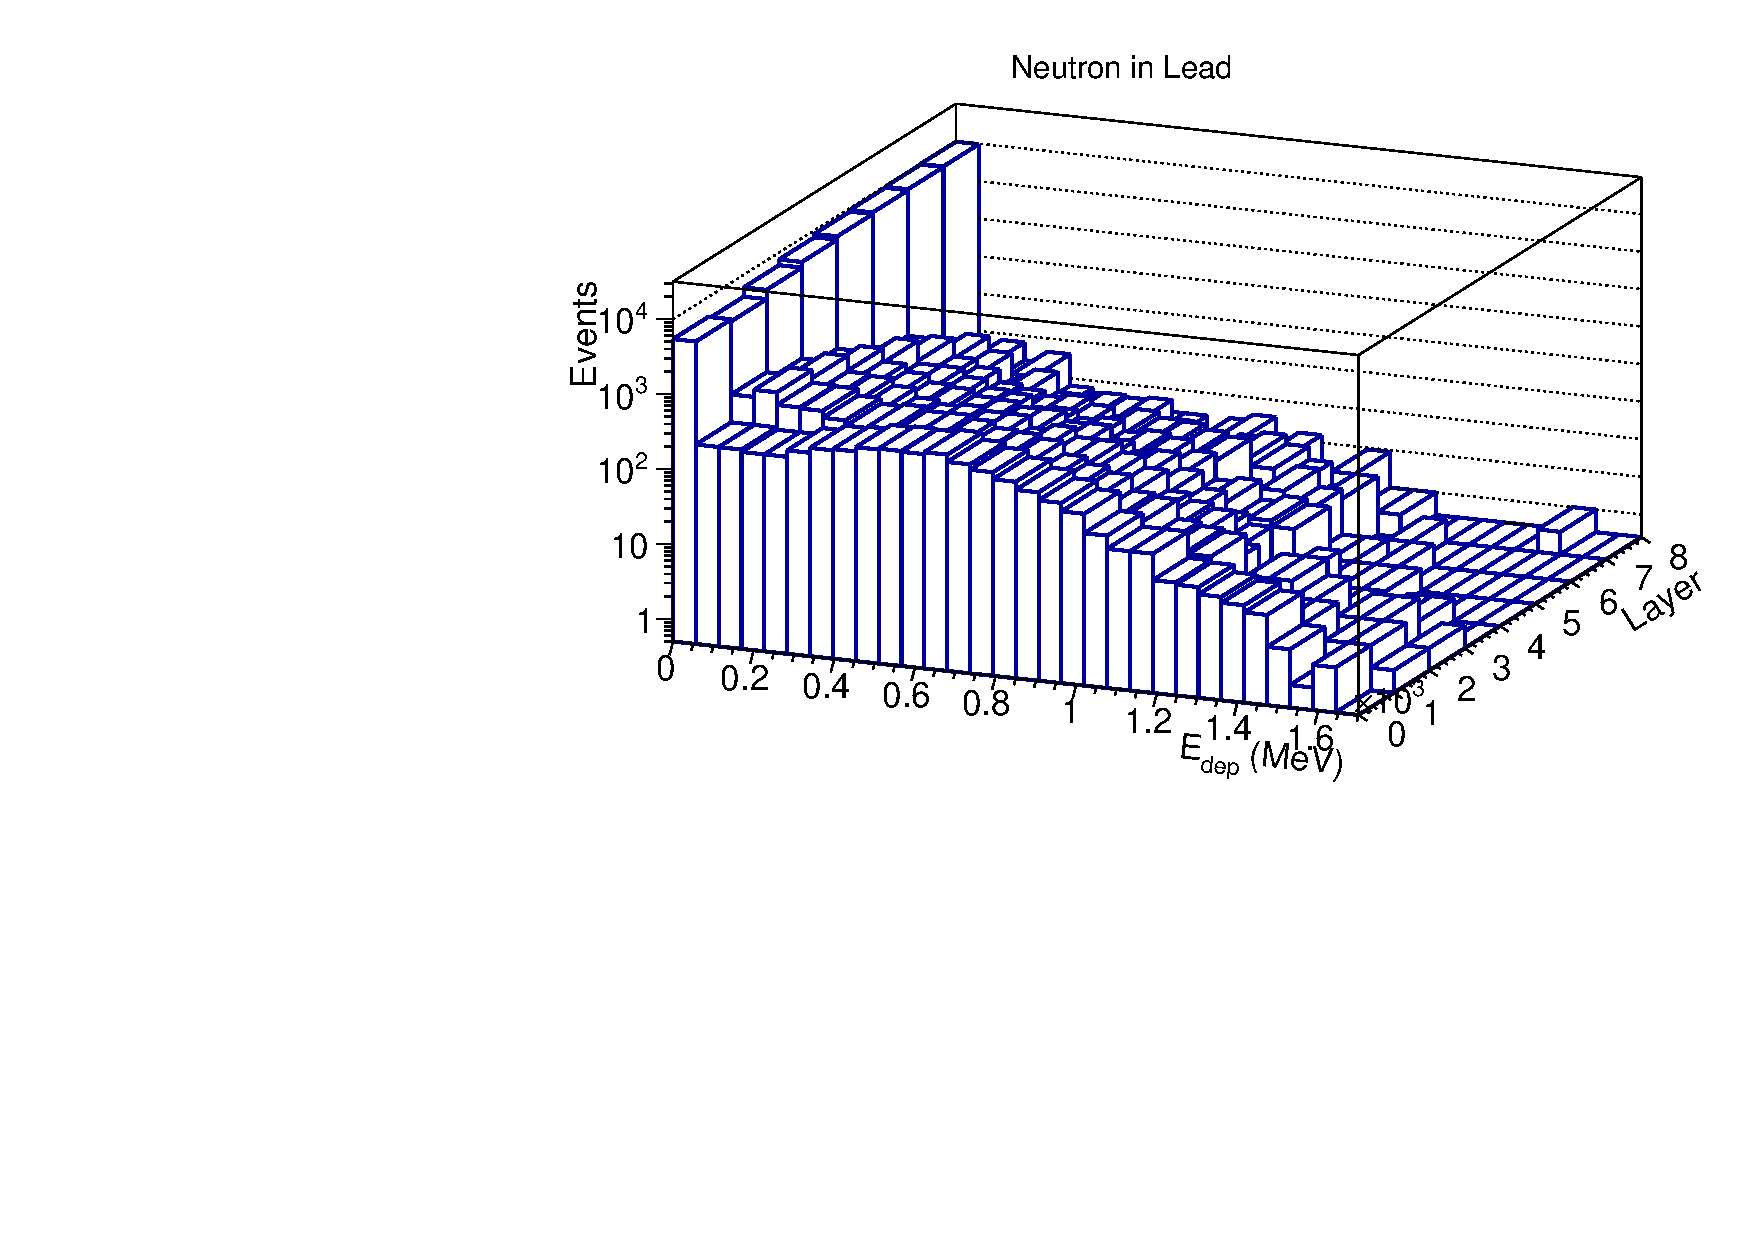
\includegraphics[width=.48\textwidth]{../report/plots/N_pb_edep.pdf}}
  \put(18.5, 60){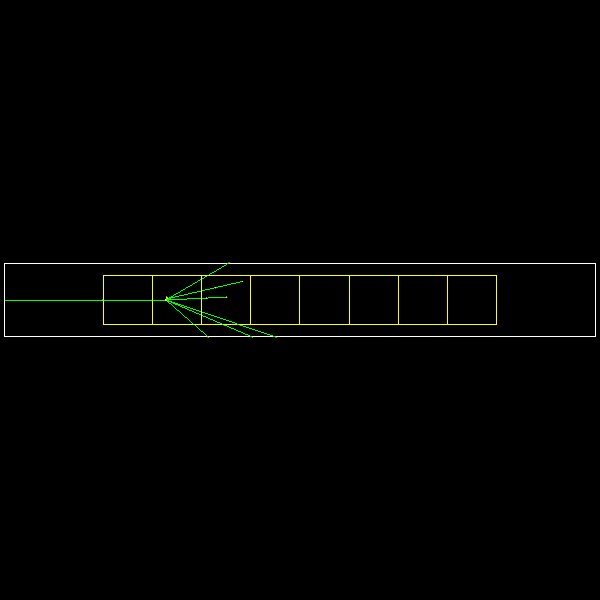
\includegraphics[width=.48\textwidth, trim = 0mm 75mm 0mm 75mm, clip]{../report/pics/N-PP.png}}
  \put(18.5, -60){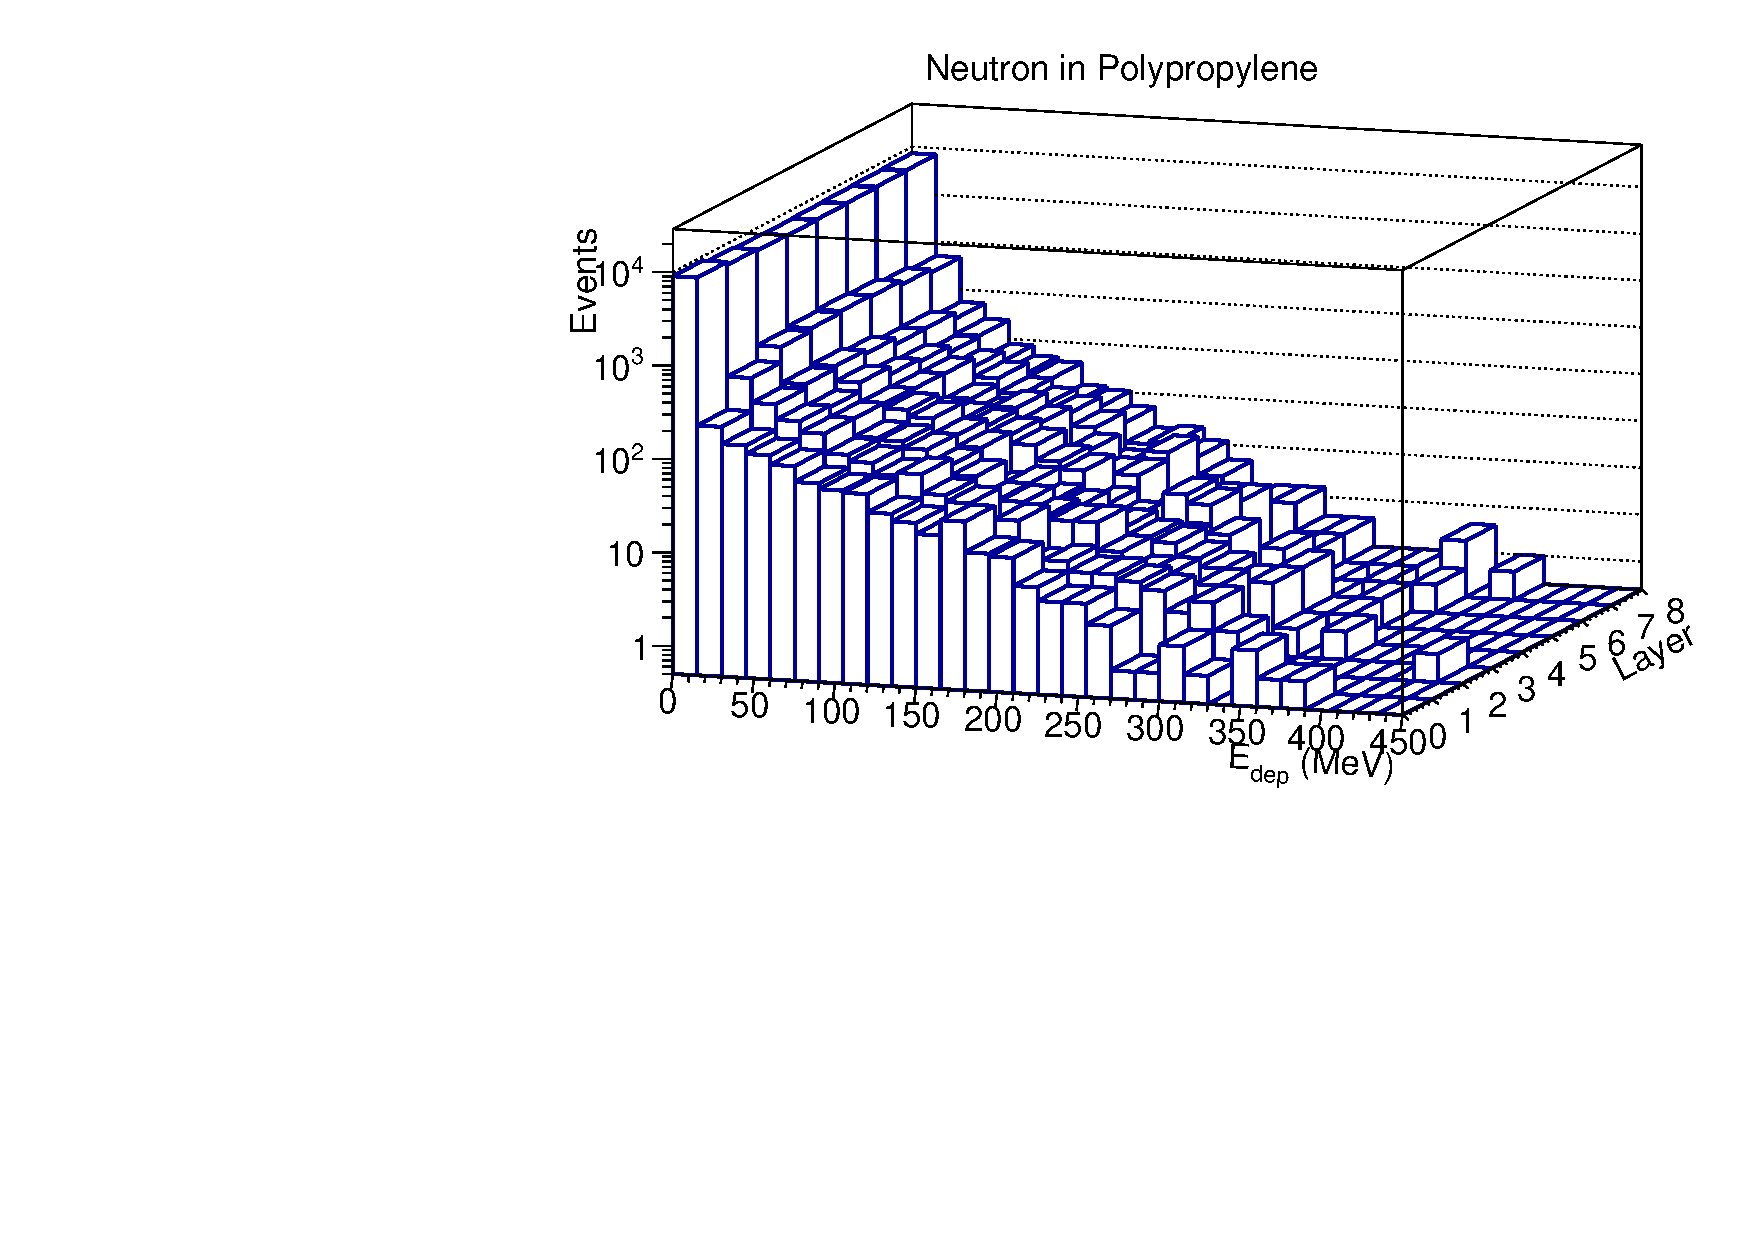
\includegraphics[width=.48\textwidth]{../report/plots/N_pp_edep.pdf}}
  \end{picture}
\end{frame}

\begin{frame}
  \frametitle{Neutron Interactions cont'd}
  \begin{picture}(320,250)(-160,-125)
  \put(-160, 60){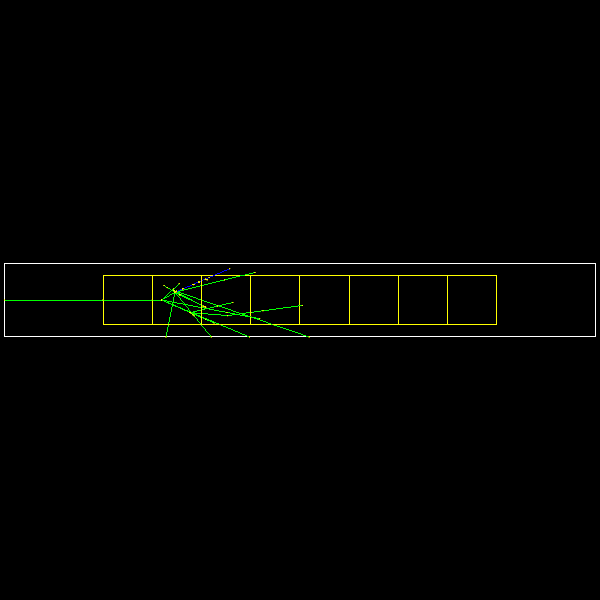
\includegraphics[width=.48\textwidth, trim = 0mm 75mm 0mm 75mm, clip]{../report/pics/N-H2O.png}}
  \put(-160, -60){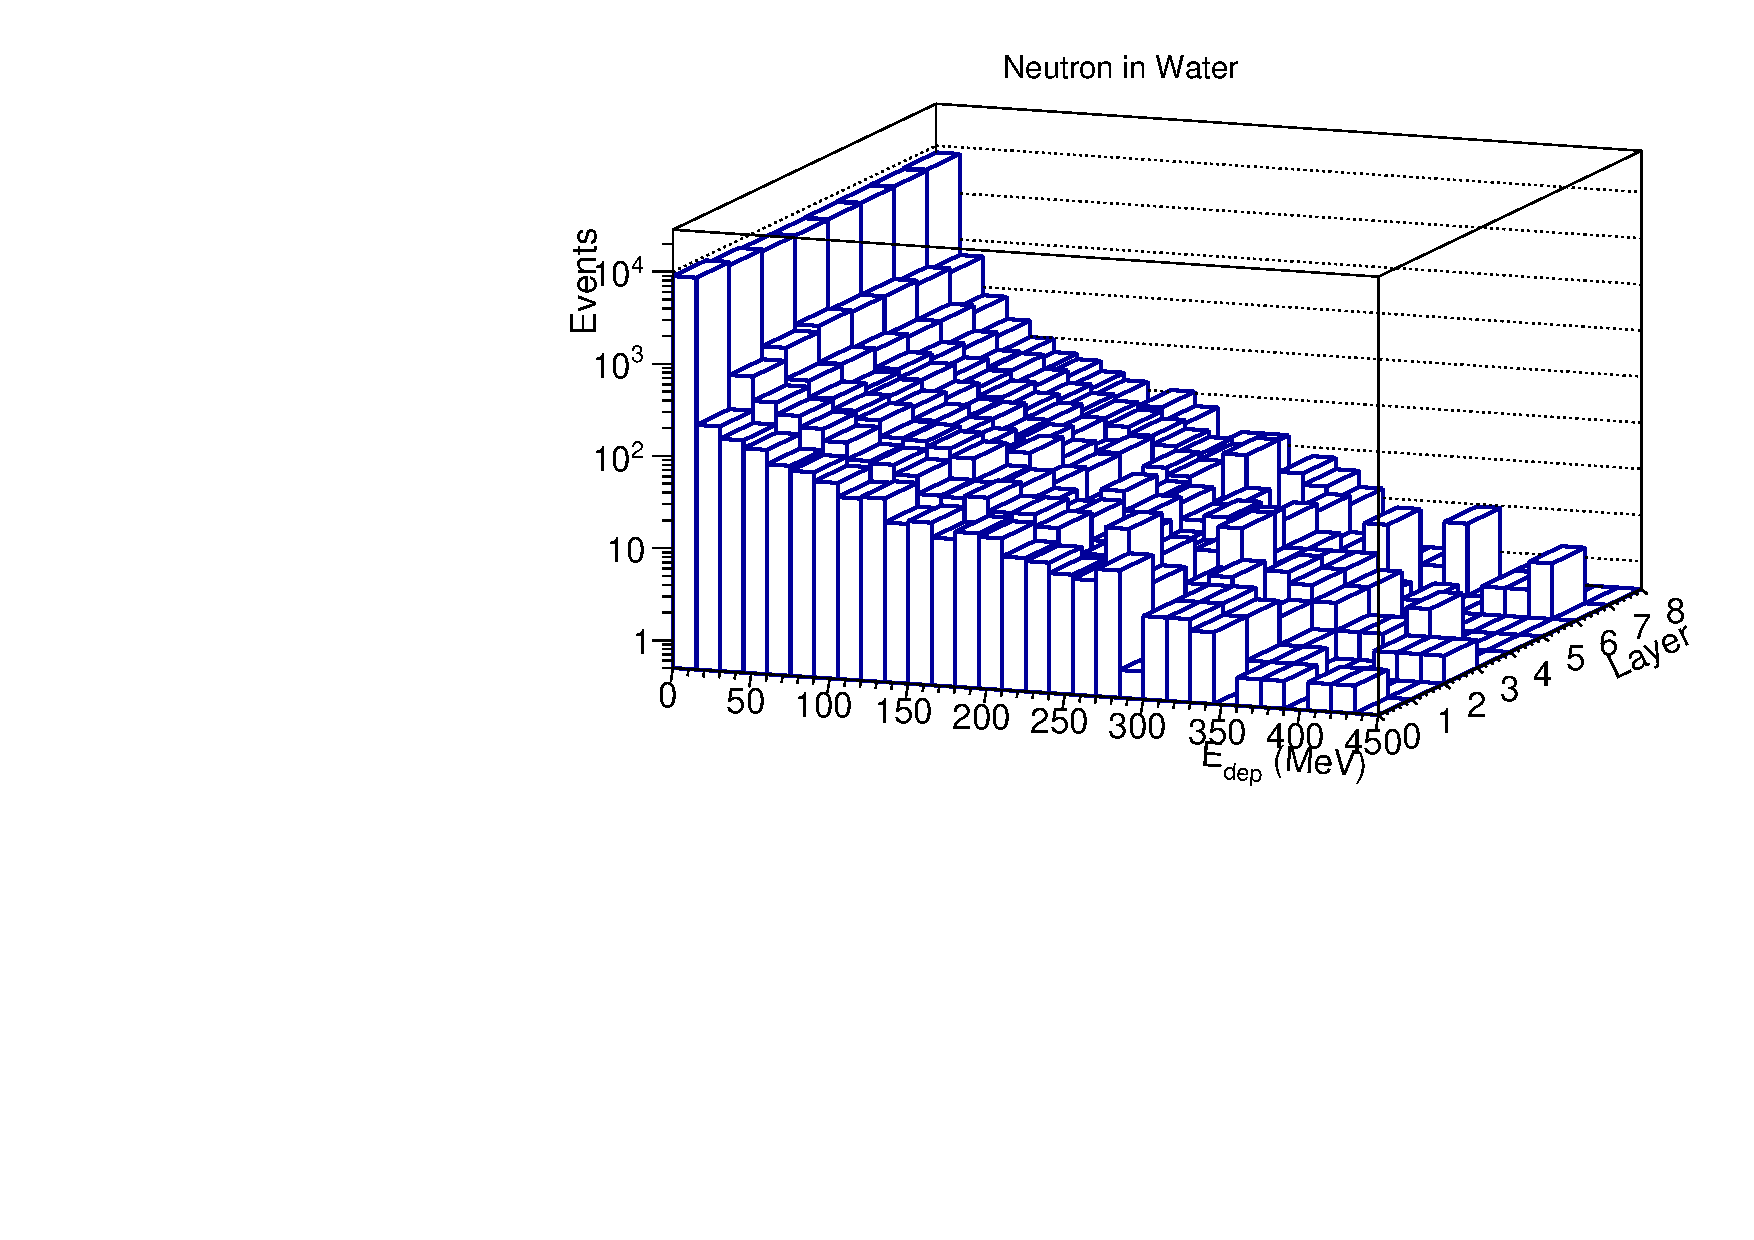
\includegraphics[width=.48\textwidth]{../report/plots/N_h2o_edep.pdf}}
  \put(18.5, -30){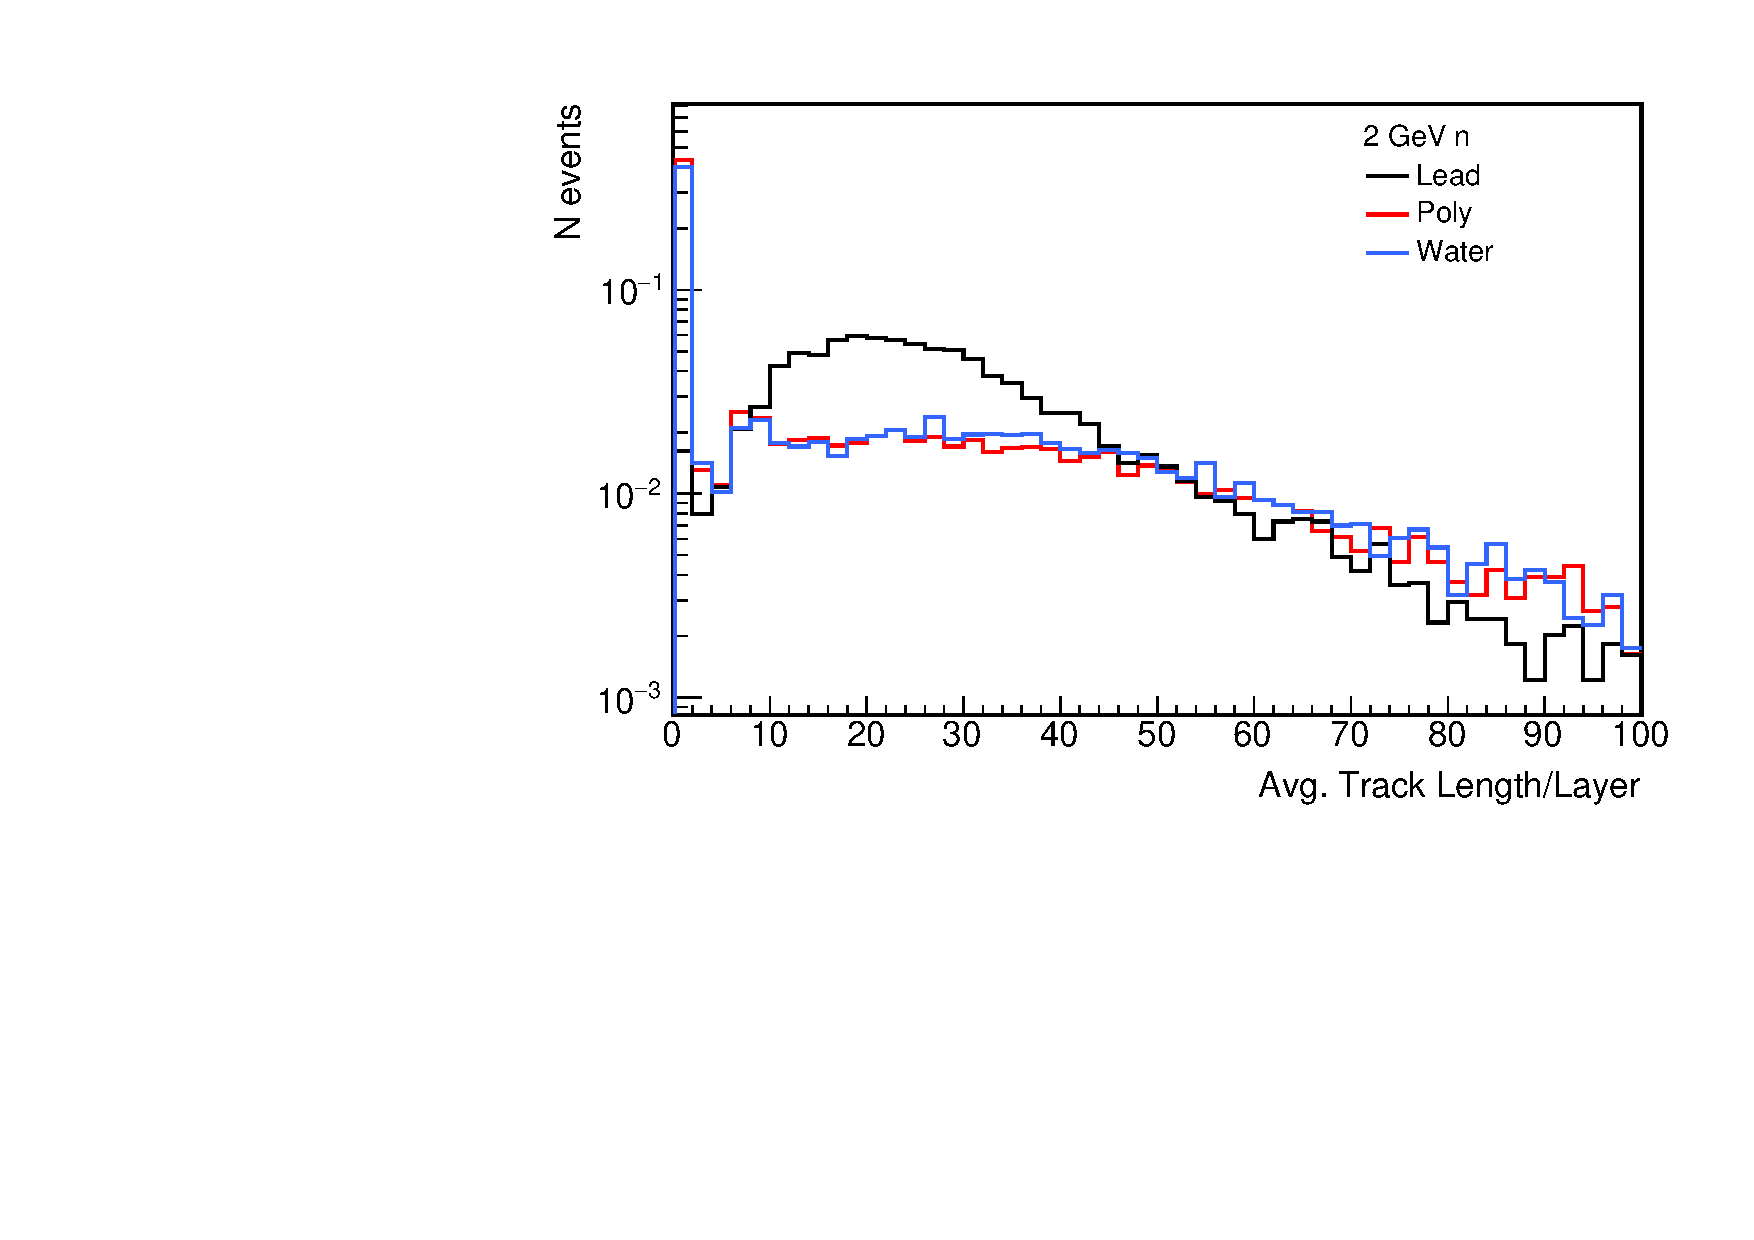
\includegraphics[width=.48\textwidth]{../report/plots/TL_neutron.pdf}}
  \end{picture}
\end{frame}


\setbeamertemplate{section page}[mine]
\section{Live Demo}


\begin{frame}
  \frametitle{Summary}
  {\footnotesize
  \begin{itemize}
    \item Geant4 is a powerful simulation tool written in C++ for many research areas (notably particle and nuclear, medical, and space physics).
    \item We discussed some of the required and major features in a Geant4 simulation program
    \item A simple simulation program was shown which was developed based on a modifed Geant4 collaboration provided example
    \item We observed interactions that are expected based on our knowledge of physics.
    \item Code for entire project: \url{http://github.com/dougphy/p1_505}
  \end{itemize}}
\end{frame}

\end{document}
